% XeLaTeX

\documentclass{article}
\usepackage{ctex}
\usepackage{xypic}
\usepackage{amsfonts,amssymb}
\usepackage{multirow}
\usepackage{geometry}
\usepackage{graphicx}
\usepackage{listings}
\usepackage{lipsum}
\usepackage{courier}
\usepackage{fancyvrb}
\usepackage{etoolbox}


\linespread{1.2}
\geometry{left=3cm,right=2.5cm,top=2.5cm,bottom=2.5cm}

\makeatletter
\patchcmd{\FV@SetupFont}
  {\FV@BaseLineStretch}
  {\fontencoding{T1}\FV@BaseLineStretch}
  {}{}
\makeatother

\lstset{basicstyle=\small\fontencoding{T1}\ttfamily,breaklines=true}
\lstset{numbers=left,frame=shadowbox,tabsize=4}
%\lstset{extendedchars=false}
\begin{document}

\title{ICPC Templates For Africamonkey}
\author {Africamonkey}
\maketitle
\tableofcontents
\newpage
\section{莫队算法}
\subsection{普通莫队}
\begin{lstlisting}[language=C++]
struct Q { int l, r, sqrtl, id; } q[N];
int n, m, v[N], ans[N], nowans;
bool cmp(const Q &a, const Q &b) {
	if (a.sqrtl != b.sqrtl) return a.sqrtl < b.sqrtl;
	return a.r < b.r;
}
void change(int x) { if (!v[x]) checkin(); else checkout(); }
int main() {
	......
	for (int i=1;i<=m;i++) q[i].sqrtl = q[i].l / sqrt(n), q[i].id = i;
	sort(q+1, q+m+1, cmp);
	int L=1,R=0; nowans=0;
	memset(v, 0, sizeof(v));
	for (int i=1;i<=m;i++) {
		while (L<q[i].l) change(L++);
		while (L>q[i].l) change(--L);
		while (R<q[i].r) change(++R);
		while (R>q[i].r) change(R--);
		ans[q[i].id] = nowans;
	}
	......
}
\end{lstlisting}
\subsection{树上莫队}

\begin{lstlisting}[language=C++]
struct Query { int l, r, id, l_group; } query[N];
struct EDGE { int adj, next; } edge[N*2];
int n, m, top, gh[N], c[N], reorder[N], deep[N], father[N], size[N], son[N], Top[N];
void addedge(int x, int y) {
	edge[++top].adj = y;
	edge[top].next = gh[x];
	gh[x] = top;
}
void dfs(int x, int root=0) {
	reorder[x] = ++top; father[x] = root; deep[x] = deep[root] + 1;
	son[x] = 0; size[x] = 1; int dd = 0;
	for (int p=gh[x]; p; p=edge[p].next)
		if (edge[p].adj != root) {
			dfs(edge[p].adj, x);
			if (size[edge[p].adj] > dd) {
				son[x] = edge[p].adj;
				dd = size[edge[p].adj];
			}
			size[x] += size[edge[p].adj];
		}
}
void split(int x, int tp) {
	Top[x] = tp;
	if (son[x]) split(son[x], tp);
	for (int p=gh[x]; p; p=edge[p].next)
		if (edge[p].adj != father[x] && edge[p].adj != son[x])
			split(edge[p].adj, edge[p].adj);
}
int lca(int x, int y) {
	int tx = Top[x], ty = Top[y];
	while (tx != ty) {
		if (deep[tx] < deep[ty]) {
			swap(tx, ty);
			swap(x, y);
		}
		x = father[tx];
		tx = Top[x];
	}
	if (deep[x] < deep[y]) swap(x, y);
	return y;
}
bool cmp(const Query &a, const Query &b) {
	if (a.l_group != b.l_group) return a.l_group < b.l_group;
	return reorder[a.r] < reorder[b.r];
}
int v[N], ans[N];
void upd(int x) { if (!v[x]) checkin(); else checkout(); }
void go(int &u, int taru, int v) {
	int lca0 = lca(u, taru);
	int lca1 = lca(u, v);	upd(lca1);
	int lca2 = lca(taru, v); upd(lca2);
	for (int x=u; x!=lca0; x=father[x]) upd(x);
	for (int x=taru; x!=lca0; x=father[x]) upd(x);
	u = taru;
}
int main() {
	memset(gh, 0, sizeof(gh));
	scanf("%d%d", &n, &m); top = 0;
	for (int i=1;i<n;i++) {
		int x,y; scanf("%d%d", &x, &y);
		addedge(x, y); addedge(y, x);
	}
	top = 0; dfs(1); split(1, 1);
	for (int i=1;i<=m;i++) {
		if (reorder[query[i].l] > reorder[query[i].r]) 
			swap(query[i].l, query[i].r);
		query[i].id = i;
		query[i].l_group = reorder[query[i].l] / sqrt(n);
	}
	sort(query+1, query+m+1, cmp);
	int L=1,R=1; upd(1);
	for (int i=1;i<=m;i++) {
		go(L,query[i].l,R);
		go(R,query[i].r,L);
		ans[query[i].id] = answer();
	}
	......
}
\end{lstlisting}

\section{字符串}
\subsection{哈希}
\begin{lstlisting}[language=C++]
const int P=31,D=1000173169;
int n, pow[N], f[N]; char a[N];
int hash(int l, int r) { return (LL)(f[r]-(LL)f[l-1]*pow[r-l+1]%D+D)%D; }
int main() {
	scanf("%d%s", &n, a+1);
	pow[0] = 1;
	for (int i=1;i<=n;i++) pow[i] = (LL)pow[i-1]*P%D;
	for (int i=1;i<=n;i++) f[i] = (LL)((LL)f[i-1]*P+a[i])%D;
}
\end{lstlisting}
\subsection{KMP}
接口: int find\_substring(char *pattern, char *text, int *next, int *ret); 

输入: 模式串,匹配串 

输出: 返回值表示模式串在匹配串中出现的次数 

KMP的next[i]表示从0到i的字符串s,前缀和后缀的最长重叠长度。
\begin{lstlisting}[language=C++]
void find_next(char *pattern, int *next) {
	int n = strlen(pattern);
	for (int i=1;i<n;i++) {
		int j = i;
		while (j > 0) {
			j = next[j];
			if (pattern[j] == pattern[i]) {
				next[i+1] = j+1;
				break;
			}
		}
	}
}
int find_substring(char *pattern, char *text, int *next, int *ret) {
	find_next(pattern, next);
	int n = strlen(pattern);
	int m = strlen(text);
	int k = 0;
	for (int i=0,j=0;i<m;i++) {
		if (j<n && text[i]==pattern[j]) {
			j++;
		} else {
			while (j>0) {
				j = next[j];
				if (text[i] == pattern[j]) {
					j++;
					break;
				}
			}
		}
		if (j == n)
			ret[k++] = i-n+1;
	}
	return k;
}
\end{lstlisting}
\subsection{可动态修改的KMP}
支持:加入一个字符,删除一个字符。

时间复杂度: $O(n \alpha)$ , $\alpha$ 为字符集大小。

代码中的字符为 $'0' - '9'$ ,可自行修改为 $'a' - 'z'$
\begin{lstlisting}[language=C++]
char t[N];
int top, nxt[N], nxt_l[N][10];
inline void del_letter() { --top; }
inline void add_letter(char x) {
	t[top++] = x;
	int j = top-1;
	memset(nxt_l[top], 0, sizeof(nxt_l[top]));
	nxt[top] = nxt_l[top-1][x-'0'];
	memcpy(nxt_l[top], nxt_l[nxt[top]], sizeof(nxt_l[nxt[top]]));
	nxt_l[top][t[nxt[top]]-'0'] = nxt[top]+1;
}
\end{lstlisting}
\subsection{扩展KMP}
接口: void ExtendedKMP(char *a, char *b, int *next, int *ret); 

输出: 

next:  a 关于自己每个后缀的最长公共前缀 

ret: a 关于 b 的每个后缀的最长公共前缀


EXKMP的next[i]表示:从i到n-1的字符串st前缀和原串前缀的最长重叠长度。

\begin{lstlisting}[language=C++]
void get_next(char *a, int *next) {
	int i, j, k;
	int n = strlen(a);
	for (j = 0; j+1<n && a[j]==a[j+1];j++);
	next[1] = j;
	k = 1;
	for (i=2;i<n;i++) {
		int len = k+next[k], l = next[i-k];
		if (l < len-i) {
			next[i] = l;
		} else {
			for (j = max(0, len-i);i+j<n && a[j]==a[i+j];j++);
			next[i] = j;
			k = i;
		}
	}
}
void ExtendedKMP(char *a, char *b, int *next, int *ret) {
	get_next(a, next);
	int n = strlen(a), m = strlen(b);
	int i, j, k;
	for (j=0;j<n && j<m && a[j]==b[j];j++);
	ret[0] = j;
	k = 0;
	for (i=1;i<m;i++) {
		int len = k+ret[k], l = next[i-k];
		if (l < len-i) {
			ret[i] = l;
		} else {
			for (j = max(0, len-i);j<n && i+j<m && a[j]==b[i+j];j++);
			ret[i] = j;
			k = i;
		}
	}
}
\end{lstlisting}

\subsection{Manacher}
p[i] 表示以 i 为对称轴的最长回文串长度
\begin{lstlisting}[language=C++]
char st[N*2], s[N];
int len, p[N*2];

while (scanf("%s", s) != EOF) {
	len = strlen(s);
	st[0] = '$', st[1] = '#';
	for (int i=1;i<=len;i++)
		st[i*2] = s[i-1], st[i*2+1] = '#';
	len = len * 2 + 2;
	int mx = 0, id = 0, ans = 0;
	for (int i=1;i<=len;i++) {
		p[i] = (mx > i) ? min(p[id*2-i]+1, mx-i) : 1;
		for (; st[i+p[i]] == st[i-p[i]]; ++p[i]) ;
		if (p[i]+i > mx) mx = p[i]+i, id = i;
		p[i] --;
		if (p[i] > ans) ans = p[i];
	}
	printf("%d\n", ans);
}
\end{lstlisting}
\subsection{最小表示法}
\begin{lstlisting}[language=C++]
string smallestRepresation(string s) {
	int i, j, k, l;
	int n = s.length();
	s += s;
	for (i=0,j=1;j<n;) {
		for (k=0;k<n && s[i+k]==s[j+k];k++);
		if (k>=n) break;
		if (s[i+k]<s[j+k]) j+=k+1;
		else {
			l=i+k;
			i=j;
			j=max(l,j)+1;
		}
	}
	return s.substr(i, n);
}
\end{lstlisting}

\subsection{AC自动机}
\begin{lstlisting}[language=C++]
struct Node {
	int next[**Size of Alphabet**];
	int terminal, fail;
} node[**Number of Nodes**];
int top;
void add(char *st) {
	int len = strlen(st), x = 1;
	for (int i=0;i<len;i++) {
		int ind = trans(st[i]);
		if (!node[x].next[ind])
			node[x].next[ind] = ++top;
		x = node[x].next[ind];
	}
	node[x].terminal = 1;
}
int q[**Number of Nodes**], head, tail;
void build() {
	head = 0, tail = 1; q[1] = 1;
	while (head != tail) {
		int x = q[++head];
		/*(when necessary) node[x].terminal |= node[node[x].fail].terminal; */
		for (int i=0;i<n;i++)
			if (node[x].next[i]) {
				if (x == 1) node[node[x].next[i]].fail = 1;
				else {
					int y = node[x].fail;
					while (y) {
						if (node[y].next[i]) {
							node[node[x].next[i]].fail = node[y].next[i];
							break;
						}
						y = node[y].fail;
					}
					if (!node[node[x].next[i]].fail) node[node[x].next[i]].fail = 1;
				}
				q[++tail] = node[x].next[i];
			}
	}
}
\end{lstlisting}

\subsection{后缀数组}
\subsubsection{倍增算法}
参数 m 表示字符集的大小,即 $0 \leq r_i < m$ 
\begin{lstlisting}[language=C++]
#define rank rank2
int n, r[N], wa[N], wb[N], ws[N], sa[N], rank[N], height[N];
int cmp(int *r, int a, int b, int l, int n) {
	if (r[a]==r[b]) {
		if (a+l<n && b+l<n && r[a+l]==r[b+l])
			return 1;
	}
	return 0;
}
void suffix_array(int m) {
	int i, j, p, *x=wa, *y=wb, *t;
	for (i=0;i<m;i++) ws[i]=0;
	for (i=0;i<n;i++) ws[x[i]=r[i]]++;
	for (i=1;i<m;i++) ws[i]+=ws[i-1];
	for (i=n-1;i>=0;i--) sa[--ws[x[i]]]=i;
	for (j=1,p=1;p<n;m=p,j<<=1) {
		for (p=0,i=n-j;i<n;i++) y[p++]=i;
		for (i=0;i<n;i++) if (sa[i]>=j) y[p++]=sa[i]-j;
		for (i=0;i<m;i++) ws[i]=0;
		for (i=0;i<n;i++) ws[x[y[i]]]++;
		for (i=1;i<m;i++) ws[i]+=ws[i-1];
		for (i=n-1;i>=0;i--) sa[--ws[x[y[i]]]]=y[i];
		for (t=x,x=y,y=t,x[sa[0]]=0,i=1,p=1;i<n;i++)
			x[sa[i]]=cmp(y,sa[i-1],sa[i],j,n)?p-1:p++;
	}
	for (i=0;i<n;i++) rank[sa[i]]=i;
	rank[n] = -1;
}
void calc_height() {
	int j=0;
	for (int i=0;i<n;i++)
		if (rank[i])
		{
			while (r[i+j]==r[sa[rank[i]-1]+j]) j++;
			height[rank[i]]=j;
			if (j) j--;
		}
}
\end{lstlisting}
\subsubsection{DC3算法}
注意:

$N$ 至少为字符串长度的 $3$ 倍

接口: suffix\_array(int *r, int *sa, int n, int m); 

r 表示字符串, sa 为后缀数组输出,$n$ 表示字符串长度,下标从 $0$ 开始。$m$ 为字符集大小。
\begin{lstlisting}[language=C++]
#define F(x) ((x)/3 + ((x)%3 == 1 ? 0:tb))
#define G(x) ((x) < tb ? (x)*3+1 : ((x)-tb)*3 + 2)
#define rank rank2

int r[N], wa[N], wb[N], ws[N], wv[N], sa[N], rank[N];

int c0(int *r,int a,int b) {
    return r[a]==r[b]&&r[a+1]==r[b+1]&&r[a+2]==r[b+2];
}

int c12(int k,int *r,int a,int b) {
    if(k==2) return r[a]<r[b]||r[a]==r[b]&&c12(1,r,a+1,b+1);
    else return r[a]<r[b]||r[a]==r[b]&&wv[a+1]<wv[b+1];
}

void dsort(int *r,int *a,int *b,int n,int m) {
    int i;for(i=0;i<n;i++) wv[i]=r[a[i]];
    for(i=0;i<m;i++) ws[i]=0;
    for(i=0;i<n;i++) ws[wv[i]]++;
    for(i=1;i<m;i++) ws[i]+=ws[i-1];
    for(i=n-1;i>=0;i--) b[--ws[wv[i]]]=a[i];
}

void dc3(int *r,int *sa,int n,int m) {
    int i,j,*rn=r+n,*san=sa+n,ta=0,tb=(n+1)/3,tbc=0,p;
    r[n]=r[n+1]=0;
    for(i=0;i<n;i++) if(i%3!=0) wa[tbc++]=i;
    dsort(r+2,wa,wb,tbc,m);
    dsort(r+1,wb,wa,tbc,m);
    dsort(r,wa,wb,tbc,m);
    for(p=1,rn[F(wb[0])]=0,i=1;i<tbc;i++) rn[F(wb[i])]=c0(r,wb[i-1],wb[i])?p-1:p++;
    if(p<tbc) dc3(rn,san,tbc,p);
    else for(i=0;i<tbc;i++) san[rn[i]]=i;
    for(i=0;i<tbc;i++) if(san[i]<tb) wb[ta++]=san[i]*3;
    if(n%3==1) wb[ta++]=n-1;
    dsort(r,wb,wa,ta,m);
    for(i=0;i<tbc;i++) wv[wb[i]=G(san[i])]=i;
    for(i=0,j=0,p=0;i<ta && j<tbc;p++)sa[p]=c12(wb[j]%3,r,wa[i],wb[j])?wa[i++]:wb[j++];
    for(;i<ta;p++) sa[p]=wa[i++];
    for(;j<tbc;p++) sa[p]=wb[j++];
}

void suffix_array(int *r, int *sa, int n, int m) {
    dc3(r, sa, n + 1, m);
    int top = 0;
    for (int i = 0; i < n + 1; ++i)
        if (sa[i] < n) sa[top++] = sa[i];
    for (int i = 0; i < n; ++i) rank[sa[i]] = i;
    rank[n] = -1;
}
\end{lstlisting}
\subsubsection{小技巧:拼接字符串}
接口: 

int gao1(int l, int r, int c, int p); 区间 $[l, r)$ 中保证第 $0$ 位到第 $c - 1$ 位都是相同的(设为字符串 $s$ ),现在我们在 $s$ 后面接一个字符 $p$ ,得到一个新的字符串 $s'$ 。返回值为最小的 $k$ 满足后缀 $sa[k]$ 前 $c + 1$ 位为 $s'$ 

int gao2(int l, int r, int c, int p); 区间 $[l, r)$ 中保证第 $0$ 位到第 $c - 1$ 位都是相同的(设为字符串 $s$ ),现在我们在 $s$ 后面接一个后缀 $sa[p]$ ,得到一个新的字符串 $s'$ 。返回值为最小的 $k$ 满足后缀 $sa[k]$ 前 $c + len(sa[p])$ 位为 $s'$ 

\begin{lstlisting}[language=C++]
int gao1(int l,int r,int c,int p) {
        --l;
        while (l+1<r) {
                int md=(l+r)>>1;
                if (sa[md]+c<n&&s[sa[md]+c]>=p) r=md; else l=md;
        }
        return r;
}
int gao2(int l,int r,int c,int p) {
        --l;
        while (l+1<r) {
                int md=(l+r)>>1;
                if (sa[md]+c<=n&&rk[sa[md]+c]>=p) r=md; else l=md;
        }
        return r;
}
\end{lstlisting}
示例调用:
\begin{lstlisting}[language=C++]
suf1[m] = -1, suf2[m] = n;
for (int i = m - 1; i >= 0; --i) {
	int l = gao1(0, n, 0, t[i]), r = gao1(0, n, 0, t[i]);
	suf1[i] = gao2(l, r, 1, suf1[i + 1]);
	suf2[i] = gao2(l, r, 1, suf2[i + 1]);
}
\end{lstlisting}
\subsection{后缀自动机}
下面的代码是求两个串的LCS(最长公共子串)。
\begin{lstlisting}[language=C++]
#include <cstdio>
#include <cstdlib>
#include <cstring>
#define N 500001
using namespace std;
char st[N];
int pre[N<<1], son[26][N<<1], step[N<<1], refer[N<<1], last, total;
int apply(int x, int now) { step[++total]=x; refer[total] = now; return total; }
void extend(char x, int now) {
	int p = last, np = apply(step[last]+1, now);
	for (; p && !son[x][p]; p=pre[p]) son[x][p] = np;
	if (!p) pre[np] = 1;
	else {
		int q = son[x][p];
		if (step[p]+1 == step[q]) pre[np] = q;
		else {
			int nq = apply(step[p]+1, now);
			for (int i=0;i<26;i++) son[i][nq] = son[i][q];
			pre[nq] = pre[q];
			pre[q] = pre[np] = nq;
			for (; p && son[x][p]==q; p=pre[p]) son[x][p] = nq;
		}
	}
	last = np;
}
void init() {
	last = total = 0;
	last = apply(0, 0);
	scanf("%s",st);
	for (int i=0; st[i]; i++)
		extend(st[i]-'a', i);
	scanf("%s",st);
}
int main() {
	init();
	int p = 1, now = 0, ans = 0;
	for (int i=0; st[i]; i++) {
		int index = st[i]-'a';
		for (; p && !son[index][p]; p = pre[p], now = step[p]) ;
		if (!p) p = 1;
		if (son[index][p]) {
			p = son[index][p];
			now++;
			if (now > ans) ans = now;
		}
	}
	printf("%d\n",ans);
	return 0;
}
\end{lstlisting}

一些定义和性质:

Right(str) 表示 str 在母串 S 中所有出现的结束位置集合

一个状态 s 表示的所有子串 Right 集合相同,为 Right(s)

Parent(s) 满足 Right(s) 是 Right(Parent(s)) 的真子集,并且 Right(Parent(s)) 的大小最小

Parent 函数可以表示一个树形结构。不妨叫它 Parent 树

一个 Right 集合和一个长度定义了一个子串

对于状态 s ,使得 Right(s) 合法的子串长度是一个区间 [min(s), max(s)]

max(Parent(s)) = min(s) - 1

令 refer(s) 表示产生 s 状态的字符所在位置。则 Right(s) 的合法子串的起始位置为 [refer(s) - max(s) + 1, refer(s) - min(s) + 1] ,即 [refer(s) - max(s) + 1, refer(s) - max(Parent(s))]

\begin{figure}[htbp]
  \centering
  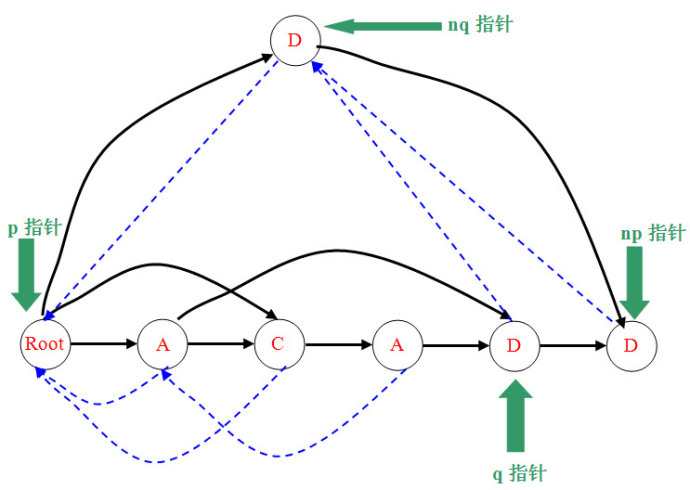
\includegraphics[scale=0.6]{suffix_auto.jpg}
  \caption{ACADD 构成的后缀自动机}
  \label{suffix_auto}
\end{figure}

我们发现 fail 构出一棵前缀树

和后缀树相同,为了使每个前缀都是叶子结点,我们不妨在串 s 前加入一个没出现的字符 '\#'

\begin{figure}
  \centering
  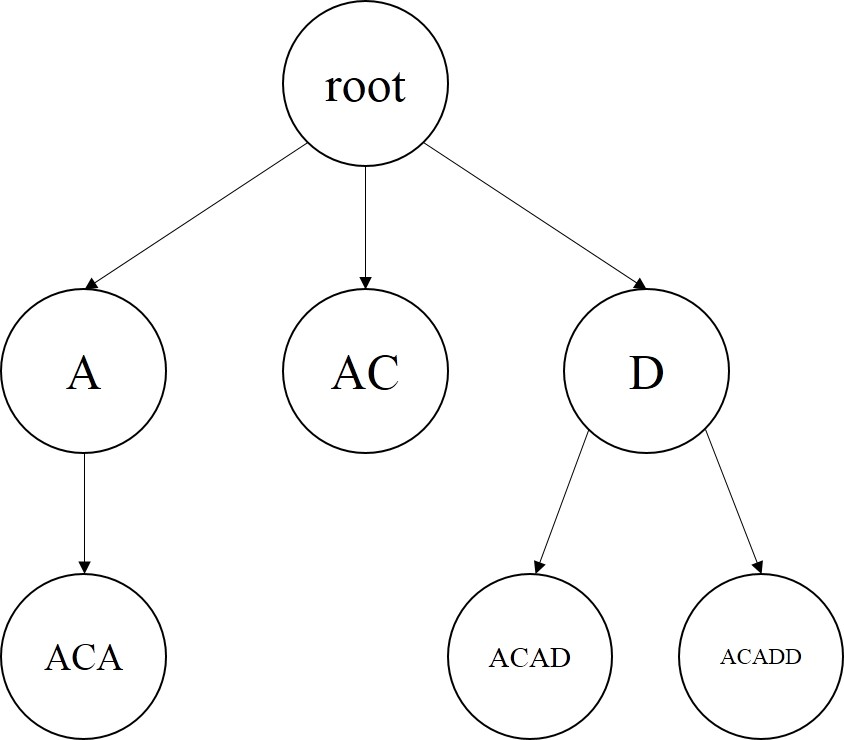
\includegraphics[scale=0.6]{suffix_auto2.jpg}
  \caption{串 ACADD 按 fail 构出的前缀树,与图 $\ref{suffix_auto}$ 对应}
  \label{suffix_auto2}
\end{figure}


\begin{figure}
  \centering
  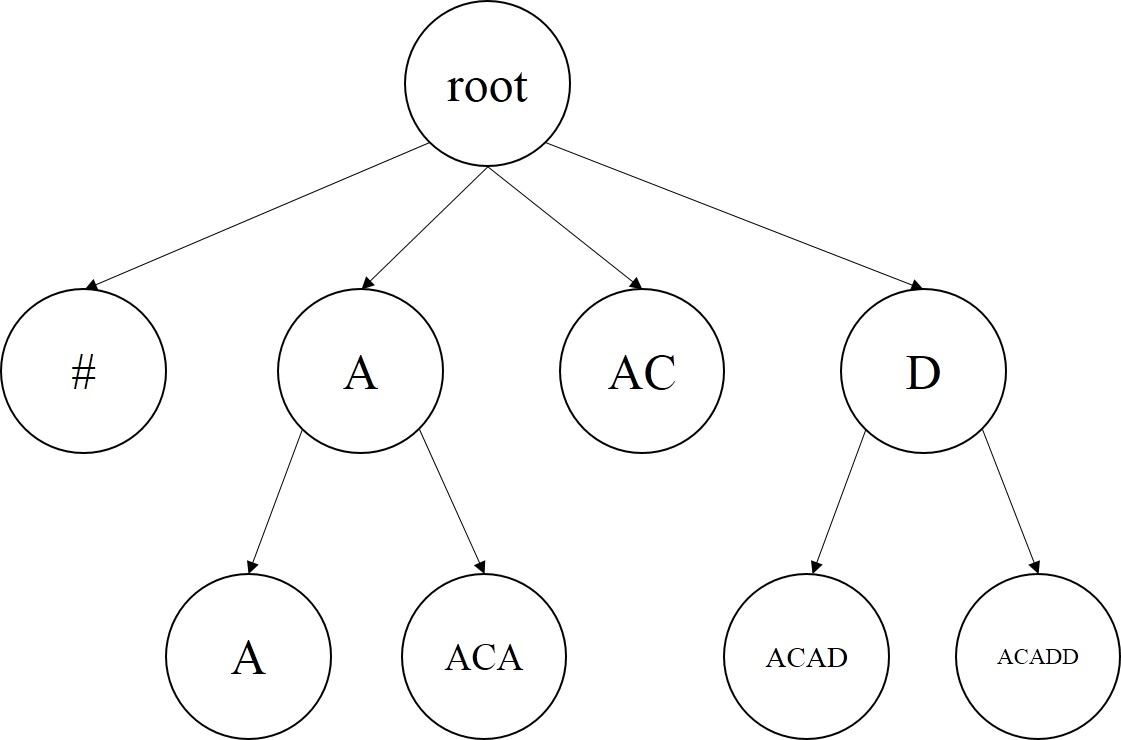
\includegraphics[scale=0.6]{suffix_auto3.jpg}
  \caption{串 \#ACADD 按 fail 构出的前缀树}
  \label{suffix_auto3}
\end{figure}

\section{数据结构}
\subsection{ST表}
\begin{lstlisting}[language=C++]
int Log[N],f[17][N];
int ask(int x,int y){
	int k=Log[y-x+1];
	return max(f[k][x],f[k][y-(1<<k)+1]);
}
int main(){
	for (int i=2;i<=n;i++)Log[i]=Log[i>>1]+1;
	for (int j=1;j<K;j++)
		for (int i=1;i+(1<<j-1)<=n;i++)
			f[j][i]=max(f[j-1][i],f[j-1][i+(1<<j-1)]);
}
\end{lstlisting}
\subsection{左偏树}

左偏树是一个可并堆。

下面的程序写的是一个小根堆,如果需要改成大根堆请在注释了 here 那行修改。

接口:

void push(const T \&x); 插入一个元素。

void merge(leftist \&x); 合并两个堆。注意,合并后原来那个堆将不可访问。

T top() const; 返回堆顶元素。

void pop(); 删除堆顶元素。

int size() const; 返回堆的大小。

\begin{lstlisting}[language=C++]
template <class T>
class leftist {
public:
    struct node {
        T key;
        int dist;
        node *l, *r;
    };
    leftist() : root(NULL), s(0) {}
    void push(const T &x) {
        leftist y;
        y.s = 1;
        y.root = new node;
        y.root -> key = x;
        y.root -> dist = 0;
        y.root -> l = y.root -> r = NULL;
        merge(y);
    }
    node* merge(node *x, node *y) {
        if (x == NULL) return y;
        if (y == NULL) return x;
        if (y -> key < x -> key) swap(x, y); //here
        x -> r = merge(x -> r, y);
        int ld = x -> l ? x -> l -> dist : -1;
        int rd = x -> r ? x -> r -> dist : -1;
        if (ld < rd) swap(x -> l, x -> r);
        if (x -> r == NULL) x -> dist = 0;
        else x -> dist = x -> r -> dist + 1;
        return x;
    }
    void merge(leftist &x) {
        root = merge(root, x.root);
        s += x.s;
    }
    T top() const {
        if (root == NULL) return T();
        return root -> key;
    }
    void pop() {
        if (root == NULL) return;
        node *p = root;
        root = merge(root -> l, root -> r);
        --s;
        delete p;
    }
    int size() const {
        return s;
    }
private:
    node* root;
    int s;
};
\end{lstlisting}
\subsection{线段树小技巧}
给定一个序列 $a$ ,寻找一个最大的 $i$ 使得 $i \leq y$ 且满足一些条件(如 $a[i] \geq w$ ,那么需要在线段树维护 $a$ 的区间最大值)
\begin{lstlisting}[language=C++]
int queryl(int p, int left, int right, int y, int w) {
	if (right <= y) {
		if (! __condition__ ) return -1;
		else if (left == right) return left;
	}
	int mid = (left + right) / 2;
	if (y <= mid) return queryl(p<<1|0, left, mid, y, w);
	int ret = queryl(p<<1|1, mid+1, right, y, w);
	if (ret != -1) return ret;
	return queryl(p<<1|0, left, mid, y, w);
}
\end{lstlisting}
给定一个序列 $a$ ,寻找一个最小的 $i$ 使得 $i \geq x$ 且满足一些条件(如 $a[i] \geq w$ ,那么需要在线段树维护 $a$ 的区间最大值)
\begin{lstlisting}[language=C++]
int queryr(int p, int left, int right, int x, int w) {
	if (left >= x) {
		if (! __condition__ ) return -1;
		else if (left == right) return left;
	}
	int mid = (left + right) / 2;
	if (x > mid) return queryr(p<<1|1, mid+1, right, x, w);
	int ret = queryr(p<<1|0, left, mid, x, w);
	if (ret != -1) return ret;
	return queryr(p<<1|1, mid+1, right, x, w);
}
\end{lstlisting}
\subsection{Splay}
接口: 

$\text{ADD x y d}$ : 将 $[x, y]$ 的所有数加上 $d$ 

$\text{REVERSE x y}$ : 将 $[x, y]$ 翻转 

$\text{INSERT x p}$ : 将 $p$ 插入到第 $x$ 个数的后面 

$\text{DEL x}$ : 将第 $x$ 个数删除
\begin{lstlisting}[language=C++]
struct SPLAY {
	struct NODE {
		int w, min;
		int son[2], size, father, rev, lazy;
	} node[N];
	int top, rt;
	void pushdown(int x) {
		if (!x) return;
		if (node[x].rev) {
			node[node[x].son[0]].rev ^= 1;
			node[node[x].son[1]].rev ^= 1;
			swap(node[x].son[0], node[x].son[1]);
			node[x].rev = 0;
		}
		if (node[x].lazy) {
			node[node[x].son[0]].lazy += node[x].lazy;
			node[node[x].son[1]].lazy += node[x].lazy;
			node[x].w += node[x].lazy;
			node[x].min += node[x].lazy;
			node[x].lazy = 0;
		}
	}
	void pushup(int x) {
		if (!x) return;
		pushdown(node[x].son[0]);
		pushdown(node[x].son[1]);
		node[x].size = node[node[x].son[0]].size + node[node[x].son[1]].size + 1;
		node[x].min = node[x].w;
		if (node[x].son[0]) node[x].min = min(node[x].min, node[node[x].son[0]].min);
		if (node[x].son[1]) node[x].min = min(node[x].min, node[node[x].son[1]].min);
	}
	void sc(int x, int y, int w) {
		node[x].son[w] = y;
		node[y].father = x;
		pushup(x);
	}
	void _ins(int w) {
		top++;
		node[top].w = node[top].min = w;
		node[top].son[0] = node[top].son[1] = 0;
		node[top].size = 1; node[top].father = 0; node[top].rev = 0;
	}
	void init() {
		top = 0;
		_ins(0); _ins(0); rt=1;
		sc(1, 2, 1);
	}
	void rotate(int x) {
		if (!x) return;
		int y = node[x].father;
		int w = node[y].son[1]==x;
		sc(y, node[x].son[w^1], w);
		sc(node[y].father, x, node[node[y].father].son[1]==y);
		sc(x, y, w^1);
	}
	int q[N];
	void flushdown(int x) {
		int t=0; for (; x; x=node[x].father) q[++t]=x;
		for (; t; t--) pushdown(q[t]);
	}
	void Splay(int x, int root=0) {
		flushdown(x);
		while (node[x].father != root) {
			int y=node[x].father;
			int w=node[y].son[1]==x;
			if (node[y].father != root && node[node[y].father].son[w]==y) rotate(y);
			rotate(x);
		}
	}
	int find(int k) {
		Splay(rt);
		while (1) {
			pushdown(rt);
			if (node[node[rt].son[0]].size+1==k) {
				Splay(rt);
				return rt;
			} else
			if (node[node[rt].son[0]].size+1<k) {
				k-=node[node[rt].son[0]].size+1;
				rt=node[rt].son[1];
			} else {
				rt=node[rt].son[0];
			}
		}
	}
	int split(int x, int y) {
		int fx = find(x);
		int fy = find(y+2);
		Splay(fx);
		Splay(fy, fx);
		return node[fy].son[0];
	}
	void add(int x, int y, int d) { //add d to each number in a[x]...a[y]
		int t = split(x, y);
		node[t].lazy += d;
		Splay(t); rt=t;
	}
	void reverse(int x, int y) { // reverse the x-th to y-th elements
		int t = split(x, y);
		node[t].rev ^= 1;
		Splay(t); rt=t;
	}
	void insert(int x, int p) { // insert p after the x-th element
		int fx = find(x+1);
		int fy = find(x+2);
		Splay(fx);
		Splay(fy, fx);
		_ins(p);
		sc(fy, top, 0);
		Splay(top); rt=top;
	}
	void del(int x) { // delete the x-th element in Splay
		int fx = find(x), fy = find(x+2);
		Splay(fx); Splay(fy, fx);
		node[fy].son[0] = 0;
		Splay(fy); rt=fy;
	}
} tree;
\end{lstlisting}

\subsection{可持久化Treap}
接口: 

void insert(int x, char c); 在当前第 $x$ 个字符后插入 $c$ 

void del(int x, int y); 删除第 $x$ 个字符到第 $y$ 个字符 

void copy(int l, int r, int x); 复制第 $l$ 个字符到第 $r$ 个字符,然后粘贴到第 $x$ 个字符后 

void reverse(int x, int y); 翻转第 $x$ 个到第 $y$ 个字符 

char query(int k); 表示询问当前第 $x$ 个字符是什么
\begin{lstlisting}[language=C++]
#define mod 1000000007
struct Treap {
	struct Node {
		char key;
		bool reverse;
		int lc, rc, size;
	} node[N];
	int n, root, rd;
	int Rand() { rd = (rd * 20372052LL + 25022087LL) % mod; return rd; }
	void init() { n = root = 0; }
	inline int copy(int x) { node[++n] = node[x]; return n; }
	inline void pushdown(int x) {
		if (!node[x].reverse) return;
		if (node[x].lc) node[x].lc = copy(node[x].lc);
		if (node[x].rc) node[x].rc = copy(node[x].rc);
		swap(node[x].lc, node[x].rc);
		node[node[x].lc].reverse ^= 1;
		node[node[x].rc].reverse ^= 1;
		node[x].reverse = 0;
	}
	inline void pushup(int x) { node[x].size = node[node[x].lc].size + node[node[x].rc].size + 1; }
	int merge(int u, int v) {
		if (!u || !v) return u+v;
		pushdown(u); pushdown(v);
		int t = Rand() % (node[u].size + node[v].size), r;
		if (t < node[u].size) {
			r = copy(u);
			node[r].rc = merge(node[u].rc, v);
		} else {
			r = copy(v);
			node[r].lc = merge(u, node[v].lc);
		}
		pushup(r);
		return r;
	}
	int split(int u, int x, int y) {
		if (x > y) return 0;
		pushdown(u);
		if (x == 1 && y == node[u].size) return u;
		if (y <= node[node[u].lc].size) return split(node[u].lc, x, y);
		int t = node[node[u].lc].size + 1;
		if (x > t) return split(node[u].rc, x-t, y-t);
		int num = copy(u);
		node[num].lc = split(node[u].lc, x, t-1);
		node[num].rc = split(node[u].rc, 1, y-t);
		pushup(num);
		return num;
	}
	void insert(int x, char c) {
		int t1 = split(root, 1, x), t2 = split(root, x+1, node[root].size);
		node[++n].key = c; node[n].size = 1;
		root = merge(merge(t1, n), t2);
	}
	void del(int x, int y) {
		int t1 = split(root, 1, x-1), t2 = split(root, y+1, node[root].size);
		root = merge(t1, t2);
	}
	void copy(int l, int r, int x) {
		int t1 = split(root, 1, x), t2 = split(root, l, r), t3 = split(root, x+1, node[root].size);
		root = merge(merge(t1, t2), t3);
	}
	void reverse(int x, int y) {
		int t1 = split(root, 1, x-1), t2 = split(root, x, y), t3 = split(root, y+1, node[root].size);
		node[t2].reverse ^= 1;
		root = merge(merge(t1, t2), t3);
	}
	char query(int k) {
		int x = root;
		while (1) {
			pushdown(x);
			if (k <= node[node[x].lc].size) x = node[x].lc;
			else 
			if (k == node[node[x].lc].size + 1) return node[x].key;
			else
			k -= node[node[x].lc].size + 1, x = node[x].rc;
		}
	}
} treap;
\end{lstlisting}
\subsection{可持久化并查集}
接口:

void init() 初始化

void merge(int x, int y, int time) 在 time 时刻将 x 和 y 连一条边,注意加边顺序必须按 time 从小到大加边

void GetFather(int x, int time) 询问 time 时刻及以前的连边状态中,x所属的集合
\begin{lstlisting}[language=C++]
namespace pers_union {
	const int inf = 0x3f3f3f3f;
	int father[N], Father[N], Time[N];
	vector<int> e[N];
	void init() {
		for (int i=1;i<=n;i++) {
			father[i] = i;
			Father[i] = i;
			Time[i] = inf;
			e[i].clear();
			e[i].push_back(i);
		}
	}
	int getfather(int x) {
		return (father[x] == x) ? x : father[x] = getfather(father[x]);
	}
	int GetFather(int x, int time) {
		return (Time[x] <= time) ? GetFather(Father[x], time) : x;
	}
	void merge(int x, int y, int time) {
		int fx = getfather(x), fy = getfather(y);
		if (fx == fy) return;
		if (e[fx].size() > e[fy].size()) swap(fx, fy);
		father[fx] = fy;
		Father[fx] = fy;
		Time[fx] = time;
		for (int i=0;i<e[fx].size();i++) {
			e[fy].push_back(e[fx][i]);
		}
	}
};
\end{lstlisting}

\section{树}
\subsection{点分治}
初始化时须设置 $top = 1$ 。
\begin{lstlisting}[language=C++]
void addedge(int x, int y) {
	edge[++top].adj = y;
	edge[top].valid = 1;
	edge[top].next = gh[x];
	gh[x] = top;
}
void get_size(int x, int root=0) {
	size[x] = 1; son[x] = 0;
	int dd = 0;
	for (int p=gh[x]; p; p=edge[p].next)
		if (edge[p].adj != root && edge[p].valid) {
			get_size(edge[p].adj, x);
			size[x] += size[edge[p].adj];
			if (size[edge[p].adj] > dd) {
				dd = size[edge[p].adj];
				son[x] = edge[p].adj;
			}
		}
}
int getroot(int x) {
	get_size(x);
	int sz = size[x];
	while (size[son[x]] > sz/2)
		x = son[x];
	return x;
}
void dc(int x) {
	x = getroot(x);
	static int list[N], ltop;
	ltop = 0;
	for (int p=gh[x]; p; p=edge[p].next)
		if (edge[p].valid)
			list[++ltop] = p;
	clear();
	for (int i=1;i<=ltop;i++) {
		update();
		modify();
	}
	clear();
	for (int i=ltop;i>=1;i--) {
		update();
		modify();
	}
	//be careful about the root
	for (int p=gh[x]; p; p=edge[p].next)
		if (edge[p].valid) {
			edge[p].valid = 0;
			edge[p^1].valid = 0;
			dc(edge[p].adj);
		}
}
\end{lstlisting}
\subsection{Link Cut Tree}
接口: 

command(x, y) : 将 x 到 y 路径的 Splay Tree 分离出来。 

linkcut(u1, v1, u2, v2) : 将树中原有的边 (u1, v1) 删除,加入一条新边 (u2, v2) 
\begin{lstlisting}[language=C++]
struct DynamicTREE{
	struct NODE{
		int father, son[2], top, size, reverse;
	} splay[N];
	void init(int i, int fat) {
		splay[i].father = splay[i].son[0] = splay[i].son[1] = 0;
		splay[i].top = fat; splay[i].size = 1; splay[i].reverse = 0;
	}
	void pushdown(int x) {
		if (!x) return;
		int s0 = splay[x].son[0], s1 = splay[x].son[1];
		if (splay[x].reverse) {
			splay[s0].reverse ^= 1;
			splay[s1].reverse ^= 1;
			swap(splay[x].son[0], splay[x].son[1]);
			splay[x].reverse = 0;
		}
		s0 = splay[x].son[0], s1 = splay[x].son[1];
		splay[s0].top = splay[s1].top = splay[x].top;
	}
	void pushup(int x) {
		if (!x) return;
		pushdown(splay[x].son[0]);
		pushdown(splay[x].son[1]);
		splay[x].size = splay[splay[x].son[0]].size + splay[splay[x].son[1]].size + 1;
	}
	void sc(int x, int y, int w, bool Auto=true) {
		splay[x].son[w] = y;
		splay[y].father = x;
		if (Auto) {
			pushup(y);
			pushup(x);
		}
	}
	int top, tush[N];
	void flowdown(int x) {
		for (top=1; x; top++, x = splay[x].father) tush[top] = x;
		for (; top; top--) pushdown(tush[top]);
	}
	void rotate(int x) {
		if (!x) return;
		int y = splay[x].father;
		int w = splay[y].son[1] == x;
		pushdown(y);
		pushdown(x);
		sc(splay[y].father, x, splay[splay[y].father].son[1]==y, false);
		sc(y, splay[x].son[w^1], w, false);
		sc(x, y, w^1, false);
		pushup(y);
		pushup(x);
	}
	void Splay(int x, int rt=0) {
		if (!x) return;
		flowdown(x);
		while (splay[x].father != rt) {
			int y = splay[x].father;
			int w = splay[y].son[1]==x;
			if (splay[y].father != rt && splay[splay[y].father].son[w] == y) rotate(y);
			rotate(x);
		}
	}
	void split(int x) {
		int y = splay[x].son[1];
		if (!y) return;
		splay[y].father = 0;
		splay[x].son[1] = 0;
		splay[y].top = x;
		pushup(x);
	}
	void access(int x) {
		int y = 0;
		while (x) {
			Splay(x);
			split(x);
			sc(x, y, 1);
			Splay(x);
			y = x;
			x = splay[x].top;
		}
	}
	void changeroot(int x) {
		access(x);
		Splay(x);
		splay[x].reverse = 1;
		Splay(x);
	}
	void command(int x, int y, ...) {
		LL ans = 0;
		changeroot(x);
		access(y);
		Splay(x);
		//then you can modify the Splay Tree
	}
	void linkcut(int u1, int v1, int u2, int v2) {
		changeroot(u1);
		access(v1);
		Splay(u1); split(u1);
		splay[v1].top = 0;
		access(u2); changeroot(u2);
		access(v2); changeroot(v2);
		Splay(u2); Splay(v2);
		splay[v2].top = u2;
	}
} lct;
\end{lstlisting}
\section{图}
\subsection{欧拉回路}
欧拉回路: 

无向图:每个顶点的度数都是偶数,则存在欧拉回路。 

有向图:每个顶点的入度 = 出度,则存在欧拉回路。 

欧拉路径: 

无向图:当且仅当该图所有顶点的度数为偶数,或者除了两个度数为奇数外其余的全是偶
数。 

有向图:当且仅当该图所有顶点出度 = 入度或者一个顶点出度 = 入度 + 1,另一个顶点入
度 = 出度 + 1,其他顶点出度 = 入度。

下面 $O(n + m)$ 求欧拉回路的代码中, $n$ 为点数, $m$ 为边数,若有解则依次输出经过的边的编号,若是无向图,则正数表示 $x$ 到 $y$ ,负数表示 $y$ 到 $x$ 。
\begin{lstlisting}[language=C++]
namespace UndirectedGraph{
	int n,m,i,x,y,d[N],g[N],v[M<<1],w[M<<1],vis[M<<1],nxt[M<<1],ed;
	int ans[M],cnt;
	void add(int x,int y,int z){
		d[x]++;
		v[++ed]=y;w[ed]=z;nxt[ed]=g[x];g[x]=ed;
	}
	void dfs(int x){
		for(int&i=g[x];i;){
			if(vis[i]){i=nxt[i];continue;}
			vis[i]=vis[i^1]=1;
			int j=w[i];
			dfs(v[i]);
			ans[++cnt]=j;
		}
	}
	void solve(){
		scanf("%d%d",&n,&m);
		for(i=ed=1;i<=m;i++)scanf("%d%d",&x,&y),add(x,y,i),add(y,x,-i);
		for(i=1;i<=n;i++)if(d[i]&1){puts("NO");return;}
		for(i=1;i<=n;i++)if(g[i]){dfs(i);break;}
		for(i=1;i<=n;i++)if(g[i]){puts("NO");return;}
		puts("YES");
		for(i=m;i;i--)printf("%d ",ans[i]);
	}
}
namespace DirectedGraph{
	int n,m,i,x,y,d[N],g[N],v[M],vis[M],nxt[M],ed;
	int ans[M],cnt;
	void add(int x,int y){
		d[x]++;d[y]--;
		v[++ed]=y;nxt[ed]=g[x];g[x]=ed;
	}
	void dfs(int x){
		for(int&i=g[x];i;){
			if(vis[i]){i=nxt[i];continue;}
			vis[i]=1;
			int j=i;
			dfs(v[i]);
			ans[++cnt]=j;
		}
	}
	void solve(){
		scanf("%d%d",&n,&m);
		for(i=1;i<=m;i++)scanf("%d%d",&x,&y),add(x,y);
		for(i=1;i<=n;i++)if(d[i]){puts("NO");return;}
		for(i=1;i<=n;i++)if(g[i]){dfs(i);break;}
		for(i=1;i<=n;i++)if(g[i]){puts("NO");return;}
		puts("YES");
		for(i=m;i;i--)printf("%d ",ans[i]);
	}
}
\end{lstlisting}
\subsection{最短路径}
\subsubsection{Dijkstra}
\begin{lstlisting}[language=C++]
#include <queue>
using namespace std;
struct EDGE { int adj, w, next; } edge[M*2];
struct dat { int id, dist; dat(int id=0, int dist=0) : id(id), dist(dist) {} };
struct cmp { bool operator () (const dat &a, const dat &b) { return a.dist > b.dist; } };
priority_queue < dat, vector<dat>, cmp > q;
int n, top, gh[N], v[N], dist[N];
void addedge(int x, int y, int w) {
	edge[++top].adj = y;
	edge[top].w = w;
	edge[top].next = gh[x];
	gh[x] = top;
}
int dijkstra(int s, int t) {
	memset(dist, 63, sizeof(dist));
	memset(v, 0, sizeof(v));
	dist[s] = 0;
	q.push(dat(s, 0));
	while (!q.empty()) {
		dat x = q.top(); q.pop();
		if (v[x.id]) continue; v[x.id] = 1;
		for (int p=gh[x.id]; p; p=edge[p].next) {
			if (x.dist + edge[p].w < dist[edge[p].adj]) {
				dist[edge[p].adj] = x.dist + edge[p].w;
				q.push(dat(edge[p].adj, dist[edge[p].adj]));
			}
		}
	}
	return dist[t];
}
\end{lstlisting}
\subsubsection{SPFA}
\begin{lstlisting}[language=C++]
struct EDGE { int adj, w, next; } edge[M*2];
int n,m,top,gh[N],v[N],cnt[N],q[N],dist[N],head,tail;
void addedge(int x, int y, int w) {
	edge[++top].adj = y;
	edge[top].w = w;
	edge[top].next = gh[x];
	gh[x] = top;
}
int spfa(int S, int T) {
	memset(v, 0, sizeof(v));
	memset(cnt, 0, sizeof(cnt));
	memset(dist, 63, sizeof(dist));
	head = 0, tail = 1;
	dist[S] = 0; q[1] = S;
	while (head != tail) {
		(head += 1) %= N;
		int x = q[head]; v[x] = 0;
		++cnt[x]; if (cnt[x] > n) return -1;
		for (int p=gh[x]; p; p=edge[p].next)
			if (dist[x] + edge[p].w < dist[edge[p].adj]) {
				dist[edge[p].adj] = dist[x] + edge[p].w;
				if (!v[edge[p].adj]) {
					v[edge[p].adj] = 1;
					(tail += 1) %= N;
					q[tail] = edge[p].adj;
				}
			}
	}
	return dist[T];
}
\end{lstlisting}
\subsection{K 短路}
接口:

kthsp::init(n) :初始化并设置节点个数为n

kthsp::add(x, y, w) :添加一条x到y的有向边

kthsp::work(S, T, k) :求S到T的第k短路
\begin{lstlisting}[language=C++]
#include <queue>
 
#define N 200020
#define M 400020
#define LOGM 20
#define LL long long
#define inf (1LL<<61)

namespace pheap {
	struct Node {
		int next, son[2];
		LL val;
	} node[M*LOGM];
	int LOG[M];
	int root[M], size[M*LOGM], top;
	int add() {
		++top; assert(top < M*LOGM);
		node[top].next = node[top].son[0] = node[top].son[1] = 0;
		node[top].val = inf;
		return top;
	}
	int copy(int x) { int t = add(); node[t] = node[x]; return t; }
	void init() {
		top = -1; add();
		for (int i=2;i<M;i++) LOG[i] = LOG[i>>1] + 1;
	}
	void upd(int x, int &next, LL &val) {
		if (val < node[x].val) {
			swap(val, node[x].val);
			swap(next, node[x].next);
		}
	}
	void insert(int x, int next, LL val) {
		int sz = size[root[x]] + 1;
		root[x] = copy(root[x]);
		size[root[x]] = sz; x = root[x];
		upd(x, next, val);
		for (int i=LOG[sz]-1;i>=0;i--) {
			int ind = (sz>>i)&1;
			node[x].son[ind] = copy(node[x].son[ind]);
			x = node[x].son[ind];
			upd(x, next, val);
		}
	}
};
 
namespace kthsp {
	using namespace pheap;
	struct EDGE {
		int adj, w, next;
	} edge[2][M];
	struct W {
		int x, y, w;
	} e[M];
	bool has_init = 0;
	int n, m, top[2], gh[2][N], v[N];
	LL dist[N];
	void init(int n1) {
		has_init = 1;
		n = n1; m = 0;
		memset(top, 0, sizeof(top));
		memset(gh, 0, sizeof(gh));
		for (int i=1;i<=n;i++) dist[i] = inf;
	}
	void addedge(int id, int x, int y, int w) {
		edge[id][++top[id]].adj = y;
		edge[id][top[id]].w = w;
		edge[id][top[id]].next = gh[id][x];
		gh[id][x] = top[id];
	}
	void add(int x, int y, int w) {
		assert(has_init);
		e[++m].x=x; e[m].y=y; e[m].w=w;
	}
	int q[N], best[N], bestw[N];
	int deg[N];
	void spfa(int S) {
		for (int i=1;i<=n;i++) deg[i] = 0;
		for (int i=1;i<=m;i++) deg[e[i].x] ++;
		int head = 0, tail = 1;
		dist[S] = 0; q[1] = S;
		while (head != tail) {
			(head += 1) %= N;
			int x = q[head];
			for (int p=gh[1][x]; p; p=edge[1][p].next) {
				if (dist[x] + edge[1][p].w < dist[edge[1][p].adj]) {
					dist[edge[1][p].adj] = dist[x] + edge[1][p].w;
					best[edge[1][p].adj] = x;
					bestw[edge[1][p].adj] = p;
				}
				if (!--deg[edge[1][p].adj]) {
					(tail += 1) %= N;
					q[tail] = edge[1][p].adj;
				}
			}
		}
	}
	void dfs(int x) {
		if (v[x]) return; v[x] = 1;
		if (best[x]) root[x] = root[best[x]];
		for (int p=gh[0][x]; p; p=edge[0][p].next)
			if (dist[edge[0][p].adj] != inf && bestw[x] != p) {
				insert(x, edge[0][p].adj, edge[0][p].w + dist[edge[0][p].adj] - dist[x]);
			}
		for (int p=gh[1][x]; p; p=edge[1][p].next)
			if (best[edge[1][p].adj] == x)
				dfs(edge[1][p].adj);
	}
	typedef pair<LL,int> pli;
	priority_queue <pli, vector<pli>, greater<pli> > pq;
	LL work(int S, int T, int k) {
		assert(has_init);
		n++; add(T, n, 0);
		if (S == T) k ++;
		T = n;
		for (int i=1;i<=m;i++) {
			addedge(0, e[i].x, e[i].y, e[i].w);
			addedge(1, e[i].y, e[i].x, e[i].w);
		}
		spfa(T);
		root[T] = 0; pheap::init();
		memset(v, 0, sizeof(v));
		dfs(T);
		while (!pq.empty()) pq.pop();
		if (k == 1) return dist[S];
		if (root[S]) pq.push(make_pair(dist[S] + node[root[S]].val, root[S]));
		while (k--) {
			if (pq.empty()) return inf;
			pli now = pq.top(); pq.pop();
			if (k == 1) return now.first;
			int x = node[now.second].next, u = node[now.second].son[0], v = node[now.second].son[1];
			if (root[x]) pq.push(make_pair(now.first + node[root[x]].val, root[x]));
			if (u) pq.push(make_pair(now.first - node[now.second].val + node[u].val, u));
			if (v) pq.push(make_pair(now.first - node[now.second].val + node[v].val, v));
		}
		return 0;
	}
};
\end{lstlisting}
\subsection{Tarjan}
割点的判断:一个顶点 $u$ 是割点,当且仅当满足 $(1)$ 或 $(2)$ : \\
$(1)$ $u$ 为树根,且 $u$ 有多于一个子树 \\
$(2)$ $u$ 不为树根,且满足存在 $(u, v)$ 为树枝边( $u$ 为 $v$ 的父亲),使得 $dfn[u] \leq low[v]$ \\
桥的判断:一条无向边 $(u, v)$ 是桥,当且仅当 $(u, v)$ 为树枝边,满足 $dfn[u] < low[v]$ 
\begin{lstlisting}[language=C++]
struct EDGE { int adj, next; } edge[M];
int n, m, top, gh[N];
int dfn[N], low[N], cnt, ind, stop, instack[N], stack[N], belong[N];
void addedge(int x, int y) {
	edge[++top].adj = y;
	edge[top].next = gh[x];
	gh[x] = top;
}
void tarjan(int x) {
	dfn[x] = low[x] = ++ind;
	instack[x] = 1; stack[++stop] = x;
	for (int p=gh[x]; p; p=edge[p].next)
		if (!dfn[edge[p].adj]) {
			tarjan(edge[p].adj);
			low[x] = min(low[x], low[edge[p].adj]);
		} else if (instack[edge[p].adj]) {
			low[x] = min(low[x], dfn[edge[p].adj]);
		}
	if (dfn[x] == low[x]) {
		++cnt; int tmp=0;
		while (tmp!=x) {
			tmp = stack[stop--];
			belong[tmp] = cnt;
			instack[tmp] = 0;
		}
	}
}
\end{lstlisting}
\subsection{2-SAT}

\begin{lstlisting}[language=C++]
#define N number_of_vertex
#define M number_of_edges

struct MergePoint {
	struct EDGE {
		int adj, next;
	} edge[M];
	int ex[M], ey[M];
	bool instack[N];
	int gh[N], top, dfn[N], low[N], cnt, ind, stop, stack[N], belong[N];
	void init() {
		cnt = ind = stop = top = 0;
		memset(dfn, 0, sizeof(dfn));
		memset(instack, 0, sizeof(instack));
		memset(gh, 0, sizeof(gh));
	}
	void addedge(int x, int y) { //reverse
		std::swap(x, y);
		edge[++top].adj = y;
		edge[top].next = gh[x];
		gh[x] = top;
		ex[top] = x;
		ey[top] = y;
	}
	void tarjan(int x) {
		dfn[x] = low[x] = ++ind;
		instack[x] = 1; stack[++stop] = x;
		for (int p=gh[x]; p; p=edge[p].next)
			if (!dfn[edge[p].adj]) {
				tarjan(edge[p].adj);
				low[x] = std::min(low[x], low[edge[p].adj]);
			} else if (instack[edge[p].adj]) {
				low[x] = std::min(low[x], dfn[edge[p].adj]);
			}
		if (dfn[x] == low[x]) {
			++cnt; int tmp = 0;
			while (tmp!=x) {
				tmp = stack[stop--];
				belong[tmp] = cnt;
				instack[tmp] = 0;
			}
		}
	}
	void work() {
		for (int i = (__first__); i <= (__last__); ++i)
			if (!dfn[i])
				tarjan(i);
	}
} merge;
 
struct Topsort {
	struct EDGE {
		int adj, next;
	} edge[M];
	int n, top, gh[N], ops[N], deg[N], ans[N];
	std::queue<int> q;
	void init() {
		n = merge.cnt; top = 0;
		memset(gh, 0, sizeof(gh));
		memset(deg, 0, sizeof(deg));
	}
	void addedge(int x, int y) {
		if (x == y) return;
		edge[++top].adj = y;
		edge[top].next = gh[x];
		gh[x] = top;
		++deg[y];
	}
	void work() {
		for (int i = 1; i <= n; ++i)
			if (!deg[i])
				q.push(i);
		while (!q.empty()) {
			int x = q.front();
			q.pop();
			for (int p = gh[x]; p; p = edge[p].next)
				if (!--deg[edge[p].adj])
					q.push(edge[p].adj);
			if (ans[x]) continue;
			ans[x] = -1; //not selected
			ans[ops[x]] = 1; //selected
		}
	}
} ts;
\end{lstlisting}
调用示例:
\begin{lstlisting}[language=C++]
	merge.init();
	merge.addedge();
	merge.work();
	for (int i = 1; i <= n; ++i) {
		if (merge.belong[U(i, 0)] == merge.belong[U(i, 1)]) {
			puts("NO");
			return 0;
		}
		ts.ops[merge.belong[U(i, 0)]] = merge.belong[U(i, 1)];
		ts.ops[merge.belong[U(i, 1)]] = merge.belong[U(i, 0)];
	}
	ts.init();
	ts.work();
	puts("YES");
	for (int i = 1; i <= n; ++i) {
		int x = U(i, 0), y = U(i, 1);
		x = merge.belong[x], y = merge.belong[y];
		x = ts.ans[x], y = ts.ans[y];
		if (x == 1) puts("0 is selected");
		if (y == 1) puts("1 is selected");
	}
\end{lstlisting}

\subsection{统治者树(Dominator Tree)}
Dominator Tree 可以解决判断一类有向图必经点的问题。

idom[x] 表示离 x 最近的必经点(重编号后)。将 idom[x] 作为 x 的父亲,构成一棵 Dominator Tree

接口:

void dominator::init(int n); 初始化,有向图节点数为 $n$ 

void dominator::addedge(int u, int v); 添加一条有向边 (u, v)

void dominator::work(int root); 以 root 为根,建立一棵 Dominator Tree 

结果的返回:

在执行 dominator::work(int root); 后,树边保存在 vector <int> tree[N] 中
\begin{lstlisting}[language=C++]
namespace dominator {
	vector <int> g[N], rg[N], bucket[N], tree[N];
	int n, ind, idom[N], sdom[N], dfn[N], dsu[N], father[N], label[N], rev[N];
	void dfs(int x) {
		++ind;
		dfn[x] = ind; rev[ind] = x;
		label[ind] = dsu[ind] = sdom[ind] = ind;
		for (auto p : g[x]) {
			if (!dfn[p]) dfs(p), father[dfn[p]] = dfn[x];
			rg[dfn[p]].push_back(dfn[x]);
		}
	}
	void init(int n1) {
		n = n1; ind = 0;
		for (int i = 1; i <= n; ++i) {
			g[i].clear();
			rg[i].clear();
			bucket[i].clear();
			tree[i].clear();
			dfn[i] = 0;
		}
	}
	void addedge(int u, int v) {
		g[u].push_back(v);
	}
	int find(int x, int step=0) {
		if (dsu[x] == x) return step ? -1 : x;
		int y = find(dsu[x], 1);
		if (y < 0) return x;
		if (sdom[label[dsu[x]]] < sdom[label[x]])
			label[x] = label[dsu[x]];
		dsu[x] = y;
		return step ? dsu[x] : label[x];
	}
	void work(int root) {
		dfs(root); n = ind;
		for (int i = n; i; --i) {
			for (auto p : rg[i])
				sdom[i] = min(sdom[i], sdom[find(p)]);
			if (i > 1) bucket[sdom[i]].push_back(i);
			for (auto p : bucket[i]) {
				int u = find(p);
				if (sdom[p] == sdom[u]) idom[p] = sdom[p];
				else idom[p] = u;
			}
			if (i > 1) dsu[i] = father[i];
		}
		for (int i = 2; i <= n; ++i) {
			if (idom[i] != sdom[i])
				idom[i] = idom[idom[i]];
			tree[rev[i]].push_back(rev[idom[i]]);
			tree[rev[idom[i]]].push_back(rev[i]);
		}
	}
};
\end{lstlisting}
\subsection{网络流}
\subsubsection{最大流}
注意: \emph{top 要初始化为 1}
\begin{lstlisting}[language=C++]
struct EDGE { int adj, w, next; } edge[M];
int n, top, gh[N], nrl[N];
void addedge(int x, int y, int w) {
	edge[++top].adj = y;
	edge[top].w = w;
	edge[top].next = gh[x];
	gh[x] = top;
	edge[++top].adj = x;
	edge[top].w = 0;
	edge[top].next = gh[y];
	gh[y] = top;
}
int dist[N], q[N];
int bfs() {
	memset(dist, 0, sizeof(dist));
	q[1] = S; int head = 0, tail = 1; dist[S] = 1;
	while (head != tail) {
		int x = q[++head];
		for (int p=gh[x]; p; p=edge[p].next)
			if (edge[p].w && !dist[edge[p].adj]) {
				dist[edge[p].adj] = dist[x] + 1;
				q[++tail] = edge[p].adj;
			}
	}
	return dist[T];
}
int dinic(int x, int delta) {
	if (x==T) return delta;
	for (int& p=nrl[x]; p && delta; p=edge[p].next)
		if (edge[p].w && dist[x]+1 == dist[edge[p].adj]) {
			int dd = dinic(edge[p].adj, min(delta, edge[p].w));
			if (!dd) continue;
			edge[p].w -= dd;
			edge[p^1].w += dd;
			return dd;
		}
	return 0;
}
int work() {
	int ans = 0;
	while (bfs()) {
		memcpy(nrl, gh, sizeof(gh));
		int t; while (t = dinic(S, inf)) ans += t;
	}
	return ans;
}
\end{lstlisting}
\subsubsection{上下界有源汇网络流}
$T$ 向 $S$ 连容量为正无穷的边,将有源汇转化为无源汇。 

每条边容量减去下界,设 $in[i]$ 表示流入 $i$ 的下界之和减去流出 $i$ 的下界之和。  

新建超级源汇 $SS, TT$ ,对于 $in[i] > 0$ 的点, $SS$ 向 $i$ 连容量为 $in[i]$ 的边。对于 $in[i] < 0$ 的点, $i$ 向 $TT$ 连容量为 $-in[i]$ 的边。 

求出以 $SS, TT$ 为源汇的最大流,如果等于 $\Sigma in[i] (in[i]>0)$ ,则存在可行流。再求出 $S, T$ 为源汇的最大流即为最大流。 

费用流:建完图后等价于求以 $SS, TT$ 为源汇的费用流。
\subsubsection{上下界无源汇网络流}
1. 怎样求无源汇有上下界网络的可行流? 

由于有源汇的网络我们先要转化成无源汇,所以本来就无源汇的网络不用再作特殊处理。 

2. 怎样求无源汇有上下界网络的最大流、最小流? 

一种简易的方法是采用二分的思想,不断通过可行流的存在与否对 $(t, s)$ 边的上下界 $U, L$ 进行调整。求最大流时令 $U = \infty$ 并二分 $L$ ;求最小流时令 $L = 0$ 并二分 $U$ 。道理很简单,因为可行流的取值范围是一段连续的区间,我们只要通过二分找到有解和无解的分界线即可。

\begin{figure}[htbp]
  \centering
  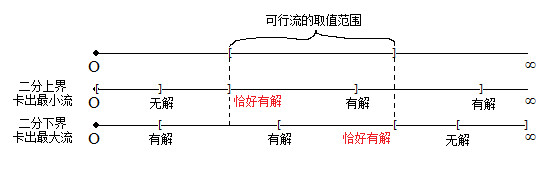
\includegraphics[scale=0.7]{nwf-1.jpg}
\end{figure}
\subsubsection{费用流}
注意: \emph{top 要初始化为 1}
\begin{lstlisting}[language=C++]
#define inf 0x3f3f3f3f
struct NetWorkFlow {
	struct EDGE {
		int adj, w, cost, next;
	} edge[M*2];
	int gh[N], q[N], dist[N], v[N], pre[N], prev[N], top;
	int S, T;
	void addedge(int x, int y, int w, int cost) {
		edge[++top].adj = y;
		edge[top].w = w;
		edge[top].cost = cost;
		edge[top].next = gh[x];
		gh[x] = top;
		edge[++top].adj = x;
		edge[top].w = 0;
		edge[top].cost = -cost;
		edge[top].next = gh[y];
		gh[y] = top;
	}
	void clear() {
		top = 1;
		memset(gh, 0, sizeof(gh));
	}
	int spfa() {
		memset(dist, 63, sizeof(dist));
		memset(v, 0, sizeof(v));
		int head = 0, tail = 1;
		q[1] = S; v[S] = 1; dist[S] = 0;
		while (head != tail) {
			(head += 1) %= N;
			int x = q[head];
			v[x] = 0;
			for (int p=gh[x]; p; p=edge[p].next)
				if (edge[p].w && dist[x] + edge[p].cost < dist[edge[p].adj]) {
					dist[edge[p].adj] = dist[x] + edge[p].cost;
					pre[edge[p].adj] = x;
					prev[edge[p].adj] = p;
					if (!v[edge[p].adj]) {
						v[edge[p].adj] = 1;
						(tail += 1) %= N;
						q[tail] = edge[p].adj;
					}
				}
		}
		return dist[T] != inf;
	}
	int work() {
		int ans = 0;
		while (spfa()) {
			int mx = inf;
			for (int x=T;x!=S;x=pre[x])
				mx = min(edge[prev[x]].w, mx);
			ans += dist[T] * mx; 
			for (int x=T;x!=S;x=pre[x]) {
				edge[prev[x]].w -= mx;
				edge[prev[x]^1].w += mx;
			}
		}
		return ans;
	}
} nwf;
\end{lstlisting}
\subsubsection{zkw费用流}
注意: \emph{top 要初始化为 1,不得用于有负权的图}
\begin{lstlisting}[language=C++]
#define inf 0x3f3f3f3f //modify if you use long long or double
template <class _tp>
struct NetWorkFlow {
	struct EDGE {
		int adj, next;
        _tp w, cost;
	} edge[M*2];
	int gh[N], top;
	int S, T;
	void addedge(int x, int y, _tp w, _tp cost) {
		edge[++top].adj = y;
		edge[top].w = w;
		edge[top].cost = cost;
		edge[top].next = gh[x];
		gh[x] = top;
		edge[++top].adj = x;
		edge[top].w = 0;
		edge[top].cost = -cost;
		edge[top].next = gh[y];
		gh[y] = top;
	}
	void clear() {
		top = 1;
		memset(gh, 0, sizeof(gh));
	}
	int v[N];
    _tp cost, d[N], slk[N];
	_tp aug(int x, _tp f) {
	    _tp left = f;
		if (x == T) {
			cost += f * d[S];
			return f;
		}
		v[x] = true;
		for (int p=gh[x]; p; p=edge[p].next)
			if (edge[p].w && !v[edge[p].adj]) {
				_tp t = d[edge[p].adj] + edge[p].cost - d[x];
				if (t == 0) {
					_tp delt = aug(edge[p].adj, min(left, edge[p].w));
					if (delt > 0) {
						edge[p].w -= delt;
						edge[p^1].w += delt;
						left -= delt;
					}
					if (left == 0) return f;
				} else {
				if (t < slk[edge[p].adj])
					slk[edge[p].adj] = t;
				}
			}
		return f-left;
	}
	bool modlabel() {
		_tp delt = inf;
		for (int i=1;i<=T;i++)
			if (!v[i]) {
				if (slk[i] < delt) delt = slk[i];
				slk[i] = inf;
			}
		if (delt == inf) return true;
		for (int i=1;i<=T;i++)
			if (v[i]) d[i] += delt;
		return false;
	}
	_tp work() {
		cost = 0;
		memset(d, 0, sizeof(d));
		memset(slk, 63, sizeof(slk));
		do {
			do {
				memset(v, 0, sizeof(v));
			} while (aug(S, inf));
		} while (!modlabel());
		return cost;
	}
};
NetWorkFlow<int> nwf;
\end{lstlisting}

\section{数学}
\subsection{扩展欧几里得解同余方程}
ans[] 保存的是循环节内所有的解
\begin{lstlisting}[language=C++]
int exgcd(int a,int b,int&x,int&y){
	if(!b)return x=1,y=0,a;
	int d=exgcd(b,a%b,x,y),t=x;
	return x=y,y=t-a/b*y,d;
}
void cal(ll a,ll b,ll n){//ax=b(mod n)
	ll x,y,d=exgcd(a,n,x,y);
	if(b%d)return;
	x=(x%n+n)%n;
	ans[cnt=1]=x*(b/d)%(n/d);
	for(ll i=1;i<d;i++)ans[++cnt]=(ans[1]+i*n/d)%n;
}
\end{lstlisting}
\subsection{同余方程组}
\begin{lstlisting} [language=C++]
int n,flag,k,m,a,r,d,x,y;
int main(){
	scanf("%d",&n);
	flag=k=1,m=0;
	while(n--){
		scanf("%d%d",&a,&r);//ans%a=r
		if(flag){
			d=exgcd(k,a,x,y);
			if((r-m)%d){flag=0;continue;}
			x=(x*(r-m)/d+a/d)%(a/d),y=k/d*a,m=((x*k+m)%y)%y;
			if(m<0)m+=y;
			k=y;
		}
	}
	printf("%d",flag?m:-1);//若flag=1,说明有解,解为ki+m,i为任意整数
}
\end{lstlisting}
\subsection{卡特兰数}
$h_1 = 1, h_n = \frac{h_{n-1}(4n-2)}{n+1} = \frac{C(2n, n)}{n+1} = C(2n, n) - C(2n, n-1)$ 

在一个格点阵列中,从 $(0, 0)$ 点走到 $(n, m)$ 点且不经过对角线 $x = y$ 的方案数 $(x > y)$ : 

$C(n+m-1, m) - C(n+m-1, m-1)$ 

在一个格点阵列中,从 $(0, 0)$ 点走到 $(n, m)$ 点且不穿过对角线 $x = y$ 的方案数 $(x \geq y)$ : 

 $C(n+m, m) - C(n+m, m-1)$ 
\subsection{斯特林数}
\subsubsection{第一类斯特林数}
第一类 Stirling 数 $S(p, k)$ 的一个组合学解释是:将 $p$ 个物体排成 $k$ 个非空循环排列的方法数。 

$S(p, k)$ 的递推公式: $S(p, k) = (p-1) S(p-1, k) + S(p-1, k-1), 1 \leq k \leq p-1$ 

边界条件: $S(p, 0) = 0, p \geq 1 \text{    } S(p, p) = 1, p \geq 0$
\subsubsection{第二类斯特林数}
第二类 Stirling 数 $S(p, k)$ 的一个组合学解释是:将 $p$ 个物体划分成 $k$ 个非空的不可辨别(可以理解为盒子没有编号)集合的方法数。

$S(p, k)$ 的递推公式: $S(p, k) = k S(p-1, k) + S(p-1, k-1), 1 \leq k \leq p-1$ 

边界条件: $S(p, 0) = 0, p \geq 1 \text{    } S(p, p) = 1, p \geq 0$

也有卷积形式: 

$$S(n, m) = \frac{1}{m!} \sum\limits_{k=0}^{m}(-1)^kC(m,k)(m-k)^n = \sum\limits_{k=0}^{m} \frac{(-1)^k(m-k)^n}{k!(m-k)!} = \sum\limits_{k=0}^{m}\frac{(-1)^k}{k!} \times \frac{(m-k)^n}{(m-k)!}$$
\subsection{错排公式}
$$D_1 = 0, D_2 = 1, D_n = (n-1)(D_{n-2} + D_{n-1})$$
\subsection{Lucas定理}
接口:  

初始化: void lucas::init(); 

计算 $C(n, m) \% mod$ 的值: LL lucas::Lucas(LL n, LL m);
\begin{lstlisting}[language=C++]
#define mod 110119
#define LL long long
namespace lucas {
	LL fac[mod+1], facv[mod+1];
	LL power(LL base, LL times) {
		LL ans = 1;
		while (times) {
			if (times&1) (ans *= base) %= mod;
			(base *= base) %= mod;
			times >>= 1;
		}
		return ans;
	}
	void init() {
		fac[0] = 1; for (int i=1;i<mod;i++) fac[i] = (fac[i-1] * i) % mod;
		facv[mod-1] = power(fac[mod-1], mod-2);
		for (int i=mod-2;i>=0;--i) facv[i] = (facv[i+1] * (i+1)) % mod;
	}
	LL C(unsigned LL n, unsigned LL m) {
		if (n < m) return 0;
		return (fac[n] * facv[m] % mod * facv[n-m] % mod) % mod;
	}
	LL Lucas(unsigned LL n, unsigned LL m)
	{
		if (m == 0) return 1;
		return (C(n%mod, m%mod) * Lucas(n/mod, m/mod)) %mod;
	}
};
\end{lstlisting}
\subsection{高斯消元}
\subsubsection{行列式}
\begin{lstlisting}[language=C++]
int ans = 1;
for (int i=0;i<n;i++) {
	for (int j=i;j<n;j++)
		if (g[j][i]) {
			for (int k=i;k<n;k++)
				swap(g[i][k], g[j][k]);
			if (j != i) ans *= -1;
			break;
		}
	if (g[i][i] == 0) {
		ans = 0;
		break;
	}
	for (int j=i+1;j<n;j++) {
		while (g[j][i]) {
			int t = g[i][i] / g[j][i];
			for (int k=i;k<n;k++)
				g[i][k] = (g[i][k] + mod - ((LL)t * g[j][k] % mod)) % mod;
			for (int k=i;k<n;k++)
				swap(g[i][k], g[j][k]);
			ans *= -1;
		}
	}
}
for (int i=0;i<n;i++)
	ans = ((LL)ans * g[i][i]) % mod;
ans = (ans % mod + mod) % mod;
printf("%d\n", ans);
\end{lstlisting}
\subsubsection{Matrix-Tree定理}
对于一张图,建立矩阵 $C$ , $C[i][i] = $ i 的度数,若 $i, j$ 之间有边,那么 $C[i][j] = -1$ ,否则为 $0$ 。这张图的生成树个数等于矩阵 $C$ 的 $n-1$ 阶行列式的值。
\subsection{调和级数}
$\sum\limits_{i=1}^n \frac{1}{i}$ 在 $n$ 较大时约等于 $ln(n) + r$ , $r$ 为欧拉常数,约等于 $0.5772156649015328$ 。
\subsection{曼哈顿距离的变换}
$\vert x_1 - x_2 \vert + \vert y_1 - y_2 \vert = max(\vert(x_1 + y_1) - (x_2 + y_2) \vert, \vert(x_1 - y_1) - (x_2 - y_2) \vert)$
\subsection{线性筛素数}
\begin{lstlisting}[language=C++]
mu[1]=phi[1]=1;top=0;
for (int i=2;i<N;i++) {
	if (!v[i]) prime[++top]=i, mu[i] = -1, phi[i] = i-1;
	for (int j=1;i*prime[j]<N && j<=top;j++) {
		v[i*prime[j]] = 1;
		if (i%prime[j]) {
			mu[i*prime[j]] = -mu[i];
			phi[i*prime[j]] = phi[i] * (prime[j]-1);
		} else {
			mu[i*prime[j]] = 0;
			phi[i*prime[j]] = phi[i] * prime[j];
			break;
		}
	}
}
\end{lstlisting}
\subsection{杜教筛}
getphi(t, x) 表示求 $\sum\limits_{i = 1}^{x} i^t \phi(i)$ 。

推导过程:

记 $S(n) = \sum\limits_{i = 1}^{n} f(i)$ ,取任意函数 $g$ 有恒等式
$$S(n) = \sum\limits_{i = 1}^{n} (f \cdot g) (i) - \sum\limits_{i = 2}^{n} g(i) S(\lfloor \frac{n}{i} \rfloor)$$

其中, $(f \cdot g)$ 表示 $f$ 和 $g$ 的狄利克雷卷积:即: $(f \cdot g) (n) = \sum\limits_{d | n} f(d)g(\frac{n}{d})$

关于恒等式的证明:

将 $\sum\limits_{i = 2}^{n} g(i)S(\lfloor \frac{n}{i} \rfloor)$ 移到左边去,即只需证

$$\sum\limits_{i = 1}^{n} (f \cdot g) (i) = \sum\limits_{i = 1}^{n} g(i) S(\lfloor \frac{n}{i} \rfloor)$$

将狄利克雷卷积展开,得:

$$\sum\limits_{i = 1}^{n} \sum\limits_{d | i} g(d) f(\frac{i}{d}) = \sum\limits_{i = 1}^{n} g(i) S(\lfloor \frac{n}{i} \rfloor)$$

即:

$$\sum\limits_{d = 1}^{n} g(d) \sum\limits_{i = 1}^{\lfloor \frac{n}{d} \rfloor} f(i) = \sum\limits_{i = 1}^{n} g(i) S(\lfloor \frac{n}{i} \rfloor)$$

显然相等,恒等式证完。

取 $f(i) = i^p \phi(i), g(i) = i^p$ ,则有:

$$S(n) = \sum\limits_{i = 1}^{n} i^p \phi(i) = \sum\limits_{i = 1}^{n} i^{p+1} - \sum\limits_{i = 2}^{n}i^pS(\lfloor \frac{n}{i} \rfloor)$$

其中有用到等式 $\sum\limits_{d | n} \phi(d) = n$

另外,莫比乌斯函数
$\mu (n) = \left\{
	\begin{array}{lr}
	1, & \text{若} n = 1 \\
	(-1)^k, & \text{若} n \text{无平方数因数,且} n = p_1p_2 \cdots p_k \\
	0, & \text{若} n \text{有大于 1 的平方数因数} \\
	\end{array}
\right.
$ 也可以使用杜教筛求前缀和,记 $S'(n) = \sum\limits_{i = 1}^{n} \mu (i)$ ,则 $S'(n) = 1 - \sum\limits_{i = 2}^{n} S'(\lfloor \frac{n}{i} \rfloor)$


\begin{lstlisting}
#include <bits/stdc++.h>
 
#define N 5000020
#define LL long long
#define mod 1000000007
#define div2 ((mod+1)/2)
#define div6 ((mod+1)/6)
 
using namespace std;
 
int n, prime[N], v[N];
LL phi[3][N];
 
map<int, int> mp[3];
 
int sum(int t, int x) { //calculate 1^t + 2^t + ... + x^t
	if (t == 0) return x;
	if (t == 1) return 1ll * x * (x + 1) % mod * div2 % mod;
	if (t == 2) return 1ll * x * (x + 1) % mod * (2ll * x % mod + 1) % mod * div6 % mod;
	if (t == 3) return 1ll * x * x % mod * (x + 1) % mod * (x + 1) % mod * div2 % mod * div2 % mod;
}
 
int getphi(int t, int x) {
	if (x < N) return phi[t][x];
	if (mp[t].find(x) != mp[t].end()) return mp[t][x];
	LL ans = 0; int r = 0;
	for (int l = 2; l <= x; l = r + 1) {
		r = x / (x / l);
		ans += 1ll * getphi(t, x / l) * (((LL)sum(t, r) - sum(t, l - 1) + mod) % mod) % mod;
		ans %= mod;
	}
	ans = (LL)sum(t + 1, x) - ans + mod;
	ans %= mod;
	mp[t][x] = ans;
	return (int)ans;
}
 
int main() {
	memset(v, 0, sizeof(v));
	int top = 0;
	phi[0][1] = 1, phi[1][1] = 1, phi[2][1] = 1;
	for (int i = 2; i < N; ++i) {
		if (!v[i]) prime[++top] = i, phi[0][i] = i - 1, phi[1][i] = 1ll * i * phi[0][i] % mod, phi[2][i] = 1ll * i * phi[1][i] % mod;
		for (int j = 1; j <= top && prime[j] * i < N; ++j) {
			v[i * prime[j]] = 1;
			if (i % prime[j] == 0) {
				phi[0][i * prime[j]] = phi[0][i] * prime[j];
				phi[1][i * prime[j]] = 1ll * phi[1][i] * prime[j] % mod * prime[j] % mod;
				phi[2][i * prime[j]] = 1ll * phi[2][i] * prime[j] % mod * prime[j] % mod * prime[j] % mod;
				break;
			} else {
				phi[0][i * prime[j]] = phi[0][i] * (prime[j] - 1);
				phi[1][i * prime[j]] = 1ll * phi[1][i] * (prime[j] - 1) % mod * prime[j] % mod;
				phi[2][i * prime[j]] = 1ll * phi[2][i] * (prime[j] - 1) % mod * prime[j] % mod * prime[j] % mod;
			}
		}
	}
	for (int i = 2; i < N; ++i) {
		phi[0][i] = (phi[0][i] + phi[0][i - 1]) % mod;
		phi[1][i] = (phi[1][i] + phi[1][i - 1]) % mod;
		phi[2][i] = (phi[2][i] + phi[2][i - 1]) % mod;
	}
}
\end{lstlisting}
\subsection{FFT}
\begin{lstlisting}[language=C++]
typedef complex<double> comp;
namespace FFT {
	comp A[N], B[N],omega[N];
	void transform(comp *x, int len) {
		for (int i=1,j=len/2;i<len-1;i++) {
			if (i<j) swap(x[i], x[j]);
			int k = len/2;
			while (j>=k) {
				j-=k;
				k/=2;
			}
			if (j<k) j+=k;
		}
	}
	void fft(comp *x, int len, int reverse) {
		transform(x, len);
		for (int h=2;h<=len;h<<=1) {
			for (int i=0;i<h/2;i++) omega[i] = polar(1.0, 2*pi*reverse/h*i);
			for (int i=0;i<len;i+=h) {
				for (int j=i;j<i+h/2;j++) {
					comp w = omega[j-i];
					comp u = x[j];
					comp v = (w * x[j+h/2]);
					x[j] = u + v;
					x[j+h/2] = u - v;
				}
			}
		}
		if (reverse == -1) {
			for (int i=0;i<len;i++)
				x[i] /= len;
		}
	}
	void work(int n, int *a, int *b) {
		int len = 1;
		while (len <= n*2) len *= 2;
		for (int i=0;i<len;i++) A[i] = B[i] = 0;
		for (int i=0;i<n;i++) A[i] = a[i], B[i] = b[i];
		fft(A, len, 1); fft(B, len, 1);
		for (int i=0;i<len;i++) A[i] = A[i] * B[i];
		fft(A, len, -1);
		for (int i=0;i<len;i++) {
			LL r = round(A[i].real());
			a[i] = r % mod;
		}
	}
};
\end{lstlisting}

\subsection{FWT}
给定长度为 $2^n$ 的序列 $A[0 \cdots 2^n-1], B[0 \cdots 2^n-1]$ ,求这两序列的

$or$ 卷积: $C_k = \sum\limits_{i \ or \ j=k} A_iB_j$

$and$ 卷积: $C_k = \sum\limits_{i \ and \ j=k} A_iB_j$

$xor$ 卷积: $C_k = \sum\limits_{i \ xor \ j=k} A_iB_j$

序列对 $10^9 + 7$ 取模
\begin{lstlisting}[language=C++]
#include <bits/stdc++.h>
using namespace std;
inline int read() {
	int s = 0; char c; while((c=getchar())<'0'||c>'9');
	do{s=s*10+c-'0';}while((c=getchar())>='0'&&c<='9');
	return s;
}
typedef long long lint;
typedef pair<lint,lint> pii;
const int N = (1<<18)+37, MO = 1e9+7;
int n;
pii tand(lint a,lint b) { return (pii){a+b,b}; }
pii iand(lint a,lint b) { return (pii){a-b,b}; }
pii tor(lint a,lint b) { return (pii){a,a+b}; }
pii ior(lint a,lint b) { return (pii){a,b-a}; }
pii txor(lint a,lint b) { return (pii){a+b,a-b}; }
pii ixor(lint a,lint b) { return (pii){(a+b)/2,(a-b)/2}; }
pii (*tr)(lint,lint);
pii (*trs[3])(lint,lint)={tor,tand,txor};
pii (*ivs[3])(lint,lint)={ior,iand,ixor};
lint a[N],b[N],x[N],y[N];
inline void fwt(lint *a) {
	int s,k,j,je;
	for(s=2;s<=n;s<<=1) for(k=0;k<n;k+=s)
		for(j=0,je=s>>1;j<je;j++) {
			pii t = tr(a[k+j],a[k+j+je]);
			a[k+j] = t.first;
			a[k+j+je] = t.second;
		}
}
int main() {
	int i;
	n = read(); n = 1<<n;
	for(i=0;i<n;i++) a[i] = read();
	for(i=0;i<n;i++) b[i] = read();
	for(int k=0;k<3;k++) {
		for(i=0;i<n;i++) x[i] = a[i], y[i] = b[i];
		tr = trs[k]; fwt(x), fwt(y);
		for(i=0;i<n;i++) x[i] *= y[i];
		tr = ivs[k]; fwt(x);
		for(i=0;i<n;i++) printf("%d ",x[i]%MO); puts("");
	}
	return 0;
}
\end{lstlisting}

\subsection{求原根}
接口: LL p\_root(LL p); 

输入: 一个素数 $p$  

输出: $p$ 的原根
\begin{lstlisting}[language=C++]
#include <bits/stdc++.h>
#define LL long long

using namespace std;

vector <LL> a;

LL pow_mod(LL base, LL times, LL mod) {
	LL ret = 1;
	while (times) {
		if (times&1) ret = ret * base % mod;
		base = base * base % mod;
		times>>=1;
	}
	return ret;
}

bool g_test(LL g, LL p) {
	for (LL i = 0; i < a.size(); ++i)
		if (pow_mod(g, (p-1)/a[i], p) == 1) return 0;
	return 1;
}

LL p_root(LL p) {
	LL tmp = p - 1;
	for (LL i = 2; i <= tmp / i; ++i)
		if (tmp % i == 0) {
			a.push_back(i);
			while (tmp % i == 0)
				tmp /= i;
		}
	if (tmp != 1) a.push_back(tmp);
	LL g = 1;
	while (1) {
		if (g_test(g, p)) return g;
		++g;
	}
}

int main() {
	LL p;
	cin >> p;
	cout << p_root(p) << endl;
}
\end{lstlisting}
\subsection{NTT}
998244353 原根为 3 , 1004535809 原根为 3 ,786433 原根为 10 , 880803841 原根为 26 。
\begin{lstlisting}[language=C++]
#define mod 998244353
#define g 3
LL wi[N], wiv[N];
LL power(LL base, LL times) {
	LL ans = 1;
	while (times) {
		if (times&1) (ans *= base) %= mod;
		(base *= base) %= mod;
		times >>= 1;
	}
	return ans;
}
void transform(LL *x, int len) {
	for (int i=1,j=len/2;i<len-1;i++) {
		if (i<j) swap(x[i], x[j]);
		int k = len/2;
		while (j>=k) {
			j-=k;
			k/=2;
		}
		if (j<k) j+=k;
	}
}
void NTT(LL *x, int len, int reverse) {
	transform(x, len);
	for (int h=2;h<=len;h<<=1) {
		for (int i=0;i<len;i+=h) {
			LL w = 1, wn;
			if (reverse==1) wn = wi[h]; else wn = wiv[h];
			for (int j=i;j<i+h/2;j++) {
				LL u = x[j];
				LL v = (w * x[j+h/2]) % mod;
				x[j	] = (u + v) % mod;
				x[j+h/2] = (u - v + mod) % mod;
				(w *= wn) %= mod;
			}
		}
	}
	if (reverse == -1) {
		LL t = power(len, mod-2);
		for (int i=0;i<len;i++)
			(x[i] *= t) %= mod;
	}
}
LL A[N], B[N];
int main() {
	for (int i=1;i<N;i*=2) {
		wi[i] = power(g, (mod-1)/i);
		wiv[i] = power(wi[i], mod-2);
	}
	memset(A, 0, sizeof(A));
	memset(B, 0, sizeof(B));
	NTT(A, len, 1); NTT(B, len, 1);
	for (int i=0;i<len;i++) (A[i] *= B[i]) %= mod;
	NTT(A, len, -1);
}
\end{lstlisting}
\subsection{组合数 lcm}
$(n+1) lcm(C(n, 0), C(n,1),...,C(n,k)) = lcm(n+1, n, n-1, ..., n-k+1)$
\subsection{区间 lcm 的维护}
对于一个数,将其分解质因数,若有因子 $p^k$ ,那么拆分出 $k$ 个数 $p, p^2, ..., p^k$ ,权值都为 $p$ ,那么查询区间 $[l, r]$ 内所有数的 lcm 的答案 = 所有在该区间中出现过的数的权值之积,可持久化线段树维护即可。

\section{几何}
\subsection{凸包}
\begin{lstlisting}[language=C++]
typedef complex<int> point;
#define X real()
#define Y imag()
int n;
long long cross(point a,point b) {
	return 1ll * a.X * b.Y - 1ll * a.Y * b.X;
}
bool cmp(point a,point b) {
	return make_pair(a.X, a.Y) < make_pair(b.X, b.Y);
}
int convexHull(point p[],int n,point ch[]) {
	sort(p, p + n, cmp);
	int m = 0;
	for(int i = 0; i < n; ++i) {
		while(m > 1 && cross(ch[m-1] - ch[m-2], p[i] - ch[m-2]) <= 0) m--;
		ch[m++] = p[i];
	}
	int k = m;
	for(int i = n - 2; i >= 0; --i) {
		while(m > k && cross(ch[m-1] - ch[m-2], p[i] - ch[m-2]) <= 0) m--;
		ch[m++] = p[i];
	}
	if(n > 1) m--;
	return m;
}
\end{lstlisting}
\section{黑科技和杂项}
\subsection{找规律}
有些题目,只给一个正整数 $n$ ,然后要求输出一个答案。这时,我们可以暴力得到小数据的解,用高斯消元得到递推式,然后用矩阵快速幂求解。

使用方法: 

首先在 gauss.in 中输入小数据的解( $n = 1$ 时, $n = 2$ 时, $\cdots$ ) ,以 $EOF$ 结束。 

依次运行 gauss.cpp , matrix.cpp ,得到 matrix.out 

将 matrix.out 中的文件粘贴在 main.cpp 中相应的位置中。注意模数一定要是质数。


\begin{lstlisting}[language=C++]
//gauss.cpp
#include <bits/stdc++.h>
#define N 102
#define mod 1000000007
//caution: you can use this program iff mod is a prime.

using namespace std;

int n, m, k, a[N], g[N][N];

int power(int base, int times) {
	int ret = 1;
	while (times) {
		if (times & 1) ret = 1ll * ret * base % mod;
		base = 1ll * base * base % mod;
		times >>= 1;
	}
	return ret;
}

int test() {
	for (int i=0;i<m;i++) {
		for (int j=i;j<=m;j++)
			if (g[j][i]) {
				for (int k=i;k<=m;k++)
					swap(g[i][k], g[j][k]);
				break;
			}
		if (g[i][i] == 0)
			return 0;
		for (int j=i+1;j<n;j++) {
			while (g[j][i]) {
				int t = 1ll * g[i][i] * power(g[j][i], mod - 2) % mod;
				for (int k=i;k<n;k++)
					g[i][k] = (g[i][k] + mod - (1ll * t * g[j][k] % mod)) % mod;
				for (int k=i;k<=m;k++)
					swap(g[i][k], g[j][k]);
			}
		}
		int t = power(g[i][i], mod - 2);
		for (int j = 0; j <= m; ++j)
			g[i][j] = 1ll * g[i][j] * t % mod;
	}
	for (int i = m; i < n; ++i)
		if (g[i][m]) return 0;
	for (int i = m - 1; i >= 0; --i) {
		int t = power(g[i][i], mod - 2);
		g[i][i] = 1;
		g[i][m] = 1ll * g[i][m] * t % mod;
		for (int j = 0; j < i; ++j)
			g[j][m] = (g[j][m] + mod - 1ll * g[i][m] * g[j][i] % mod) % mod;
	}
	printf("%d\n", m);
	for (int i = 0; i < m; ++i)
		printf("%d ", g[i][m]);
	puts("");
	for (int i = 0; i < m - 1; ++i)
		printf("%d ", a[i]);
	puts("1");
	return 1;
}

int main() {
	freopen("gauss.in", "r", stdin);
	freopen("gauss.out", "w", stdout);
	k = 0;
	while (~scanf("%d", &a[k++])) ;
	for (int sm = 1; sm <= k - sm; ++sm) {
		n = k - sm - 1;
		m = sm + 1;
		for (int i = 0; i < n; ++i) {
			for (int j = 0; j <= sm; ++j)
				g[i][j] = a[i + j];
			g[i][m] = 1;
			swap(g[i][m - 1], g[i][m]);
		}
		if (test()) return 0;
	}
	puts("no solution");
	return 0;
}
\end{lstlisting}

\begin{lstlisting}[language=C++]
//matrix.cpp
#include <bits/stdc++.h>
#define N 102
using namespace std;

int n, a[N];

int main() {
    freopen("gauss.out", "r", stdin);
    freopen("matrix.out", "w", stdout);
    scanf("%d", &n);
    for (int i = 0; i < n; ++i) scanf("%d", &a[i]);
    printf("#define M %d\n", n);
    printf("const int trans[M][M] = {\n");
    for (int i = 0; i < n; ++i) {
        printf("\t{");
        for (int j = 0; j < n; ++j) {
            int t;
            if (j < n - 2) t = i == j + 1;
            else if (j == n - 2) t = a[i];
            else t = i == n - 1;
            printf("%s%d", j == 0 ? "" : ", ", t);
        }
        printf("}%s\n", i == n - 1 ? "" : ",");
    }
    printf("};\n");
    printf("const int pref[M] = {");
    for (int i = 0; i < n; ++i) {
        int x;
        scanf("%d", &x);
        printf("%d%s", x, i == n - 1 ? "};\n" : ", ");
    }
    return 0;
}
\end{lstlisting}

\begin{lstlisting}[language=C++]
//main.cpp
#include <bits/stdc++.h>
using namespace std;

/* paste matrix.out here. */

#define mod 1000000007

struct Matrix {
    int c[M][M];
    void clear() { memset(c, 0, sizeof(c)); }
    void identity() { clear(); for (int i = 0; i < M; ++i) c[i][i] = 1; }
    void base() { memcpy(c, trans, sizeof(trans)); }
    friend Matrix operator * (const Matrix &a, const Matrix &b) {
        Matrix c; c.clear();
        for (int i = 0; i < M; ++i)
            for (int j = 0; j < M; ++j)
                for (int k = 0; k < M; ++k)
                    c.c[i][j] = (c.c[i][j] + 1ll * a.c[i][k] * b.c[k][j] % mod) % mod;
        return c;
    }
} start, base;

Matrix power(Matrix base, int times) {
    Matrix ret; ret.identity();
    while (times) {
        if (times & 1) ret = ret * base;
        base = base * base;
        times >>= 1;
    }
    return ret;
}

int main() {
    int tot;
    scanf("%d", &tot);
    while (tot--) {
        int n;
        scanf("%d", &n);
        start.clear();
        for (int i = 0; i < M; ++i) start.c[0][i] = pref[i];
        base.base();
        base = power(base, n - 1);
        start = start * base;
        printf("%d\n", start.c[0][0]);
    }
    return 0;
}
\end{lstlisting}

\subsection{高精度计算}
\begin{lstlisting}[language=C++]
#include<algorithm>
using namespace std;
const int N_huge=850,base=100000000;
char s[N_huge*10];
struct huge{
	typedef long long value;
	value a[N_huge];int len;
	void clear(){len=1;a[len]=0;}
	huge(){clear();}
	huge(value x){*this=x;}
	huge operator =(huge b){
		len=b.len;for (int i=1;i<=len;++i)a[i]=b.a[i]; return *this;
	}
	huge operator =(value x){
		len=0;
		while (x)a[++len]=x%base,x/=base;
		if (!len)a[++len]=0;
		return *this;
	}
	huge operator +(huge b){
		int L=len>b.len?len:b.len;huge tmp;
		for (int i=1;i<=L+1;++i)tmp.a[i]=0;
		for (int i=1;i<=L;++i){
			if (i>len)tmp.a[i]+=b.a[i];
			else if (i>b.len)tmp.a[i]+=a[i];
			else {
				tmp.a[i]+=a[i]+b.a[i];
				if (tmp.a[i]>=base){
					tmp.a[i]-=base;++tmp.a[i+1];
				}
			}
		}
		if (tmp.a[L+1])tmp.len=L+1;
			else tmp.len=L;
		return tmp;
	}
	huge operator -(huge b){
		int L=len>b.len?len:b.len;huge tmp;
		for (int i=1;i<=L+1;++i)tmp.a[i]=0;
		for (int i=1;i<=L;++i){
			if (i>b.len)b.a[i]=0;
			tmp.a[i]+=a[i]-b.a[i];
			if (tmp.a[i]<0){
				tmp.a[i]+=base;--tmp.a[i+1];
			}
		}
		while (L>1&&!tmp.a[L])--L;
		tmp.len=L;
		return tmp;
	}
	huge operator *(huge b){
		int L=len+b.len;huge tmp;
		for (int i=1;i<=L;++i)tmp.a[i]=0;
		for (int i=1;i<=len;++i)
			for (int j=1;j<=b.len;++j){
				tmp.a[i+j-1]+=a[i]*b.a[j];
				if (tmp.a[i+j-1]>=base){
					tmp.a[i+j]+=tmp.a[i+j-1]/base;
					tmp.a[i+j-1]%=base;
				}
			}
		tmp.len=len+b.len;
		while (tmp.len>1&&!tmp.a[tmp.len])--tmp.len;
		return tmp;
	}
	pair<huge,huge> divide(huge a,huge b){
		int L=a.len;huge c,d;
		for (int i=L;i;--i){
		c.a[i]=0;d=d*base;d.a[1]=a.a[i];
			int l=0,r=base-1,mid;
			while (l<r){
				mid=(l+r+1)>>1;
				if (b*mid<=d)l=mid;
					else r=mid-1;
			}
			c.a[i]=l;d-=b*l;
		}
		while (L>1&&!c.a[L])--L;c.len=L;
		return make_pair(c,d);
	}
	huge operator /(value x){
		value d=0;huge tmp;
		for (int i=len;i;--i){
			d=d*base+a[i];
			tmp.a[i]=d/x;d%=x;
		}
		tmp.len=len;
		while (tmp.len>1&&!tmp.a[tmp.len])--tmp.len;
		return tmp;
	}
	value operator %(value x){
		value d=0;
		for (int i=len;i;--i)d=(d*base+a[i])%x;
		return d;
	}
	huge operator /(huge b){return divide(*this,b).first;}
	huge operator %(huge b){return divide(*this,b).second;}
	huge &operator +=(huge b){*this=*this+b;return *this;}
	huge &operator -=(huge b){*this=*this-b;return *this;}
	huge &operator *=(huge b){*this=*this*b;return *this;}
	huge &operator ++(){huge T;T=1;*this=*this+T;return *this;}
	huge &operator --(){huge T;T=1;*this=*this-T;return *this;}
	huge operator ++(int){huge T,tmp=*this;T=1;*this=*this+T;return tmp;}
	huge operator --(int){huge T,tmp=*this;T=1;*this=*this-T;return tmp;}
	huge operator +(value x){huge T;T=x;return *this+T;}
	huge operator -(value x){huge T;T=x;return *this-T;}
	huge operator *(value x){huge T;T=x;return *this*T;}
	huge operator *=(value x){*this=*this*x;return *this;}
	huge operator +=(value x){*this=*this+x;return *this;}
	huge operator -=(value x){*this=*this-x;return *this;}
	huge operator /=(value x){*this=*this/x;return *this;}
	huge operator %=(value x){*this=*this%x;return *this;}
	bool operator ==(value x){huge T;T=x;return *this==T;}
	bool operator !=(value x){huge T;T=x;return *this!=T;}
	bool operator <=(value x){huge T;T=x;return *this<=T;}
	bool operator >=(value x){huge T;T=x;return *this>=T;}
	bool operator <(value x){huge T;T=x;return *this<T;}
	bool operator >(value x){huge T;T=x;return *this>T;}
	bool operator <(huge b){
		if (len<b.len)return 1;
		if (len>b.len)return 0;
		for (int i=len;i;--i){
			if (a[i]<b.a[i])return 1;
			if (a[i]>b.a[i])return 0;
		}
		return 0;
	}
	bool operator ==(huge b){
		if (len!=b.len)return 0;
		for (int i=len;i;--i)
			if (a[i]!=b.a[i])return 0;
		return 1;
	}
	bool operator !=(huge b){return !(*this==b);}
	bool operator >(huge b){return !(*this<b||*this==b);}
	bool operator <=(huge b){return (*this<b)||(*this==b);}
	bool operator >=(huge b){return (*this>b)||(*this==b);}
	void str(char s[]){
		int l=strlen(s);value x=0,y=1;len=0;
		for (int i=l-1;i>=0;--i){
			x=x+(s[i]-'0')*y;y*=10;
			if (y==base)a[++len]=x,x=0,y=1;
		}
		if (!len||x)a[++len]=x;
	}
	void read(){
		scanf("%s",s);this->str(s);
	}
	void print(){
		printf("%d",(int)a[len]);
		for (int i=len-1;i;--i){
			for (int j=base/10;j>=10;j/=10){
				if (a[i]<j)printf("0");
					else break;
			}
			printf("%d",(int)a[i]);
		}
		printf("\n");
	}
}f[1005];
int main(){
	f[1]=f[2]=1;
	for(int i=3;i<=1000;i++)f[i]=f[i-1]+f[i-2];
}
\end{lstlisting}

\subsection{读入优化}
\begin{lstlisting}[language=C++]
#define rd RD<int>
#define rdll RD<long long>
template <typename Type>
inline Type RD() {
    Type x = 0;
    int flag = 0;
    char c = getchar();
    while (!isdigit(c) && c != '-')
        c = getchar();
    (c == '-') ? (flag = 1) : (x = c - '0');
    while (isdigit(c = getchar()))
        x = x * 10 + c - '0';
    return flag ? -x : x;
}
inline char rdch() {
    char c = getchar();
    while (!isalpha(c)) c = getchar();
    return c;
}
\end{lstlisting}

\subsection{位运算及其运用}

\subsubsection{枚举子集}

枚举 $i$ 的非空子集 $j$

\begin{lstlisting}[language=C++]
for (int j = i; j; j = (j - 1) & i);
\end{lstlisting}

\subsubsection{求 1 的个数}

\begin{lstlisting}[language=C++]
int __builtin_popcount(unsigned int x);
\end{lstlisting}

\subsubsection{求前缀 0 的个数}

\begin{lstlisting}[language=C++]
int __builtin_clz(unsigned int x);
\end{lstlisting}

\subsubsection{求后缀 0 的个数}

\begin{lstlisting}[language=C++]
int __builtin_ctz(unsigned int x);
\end{lstlisting}


\end{document}
















